\chapter{RRTFunnel}

\section{Funnel}

\subsection{Funnel library}

\subsection{Creating suitable funnels}

The funnels

\subsection{Nominal trajectories}

Generating the nominal trajectories is done through the \textit{Direct
  Collocation method}, as shown in \cite{DirectCollocation paper}.

\subsubsection{Richness of the funnel library}

Currently we only have three motion primitives in our motion libray. One left
motion, one straight, and one right, which is the symmetrical opposite of the
left motion. 

\section{Uncertainty}

\subsection{Effects of degree of uncertainty}

The RRTFunnel algorithm relies upon a set of precomputed funnels which have some
uncertainty robustness already built in, although the uncertainty has to be bounded.

\section{Distance metric}

\subsection{Euclidean distance metric}

The simplest mestric used is the euclidean distance metric. Here both the
closest node in the tree, and the local extension function use the euclidean
distance metric, which shows some significant shortfalls. As an example:

\begin{figure}
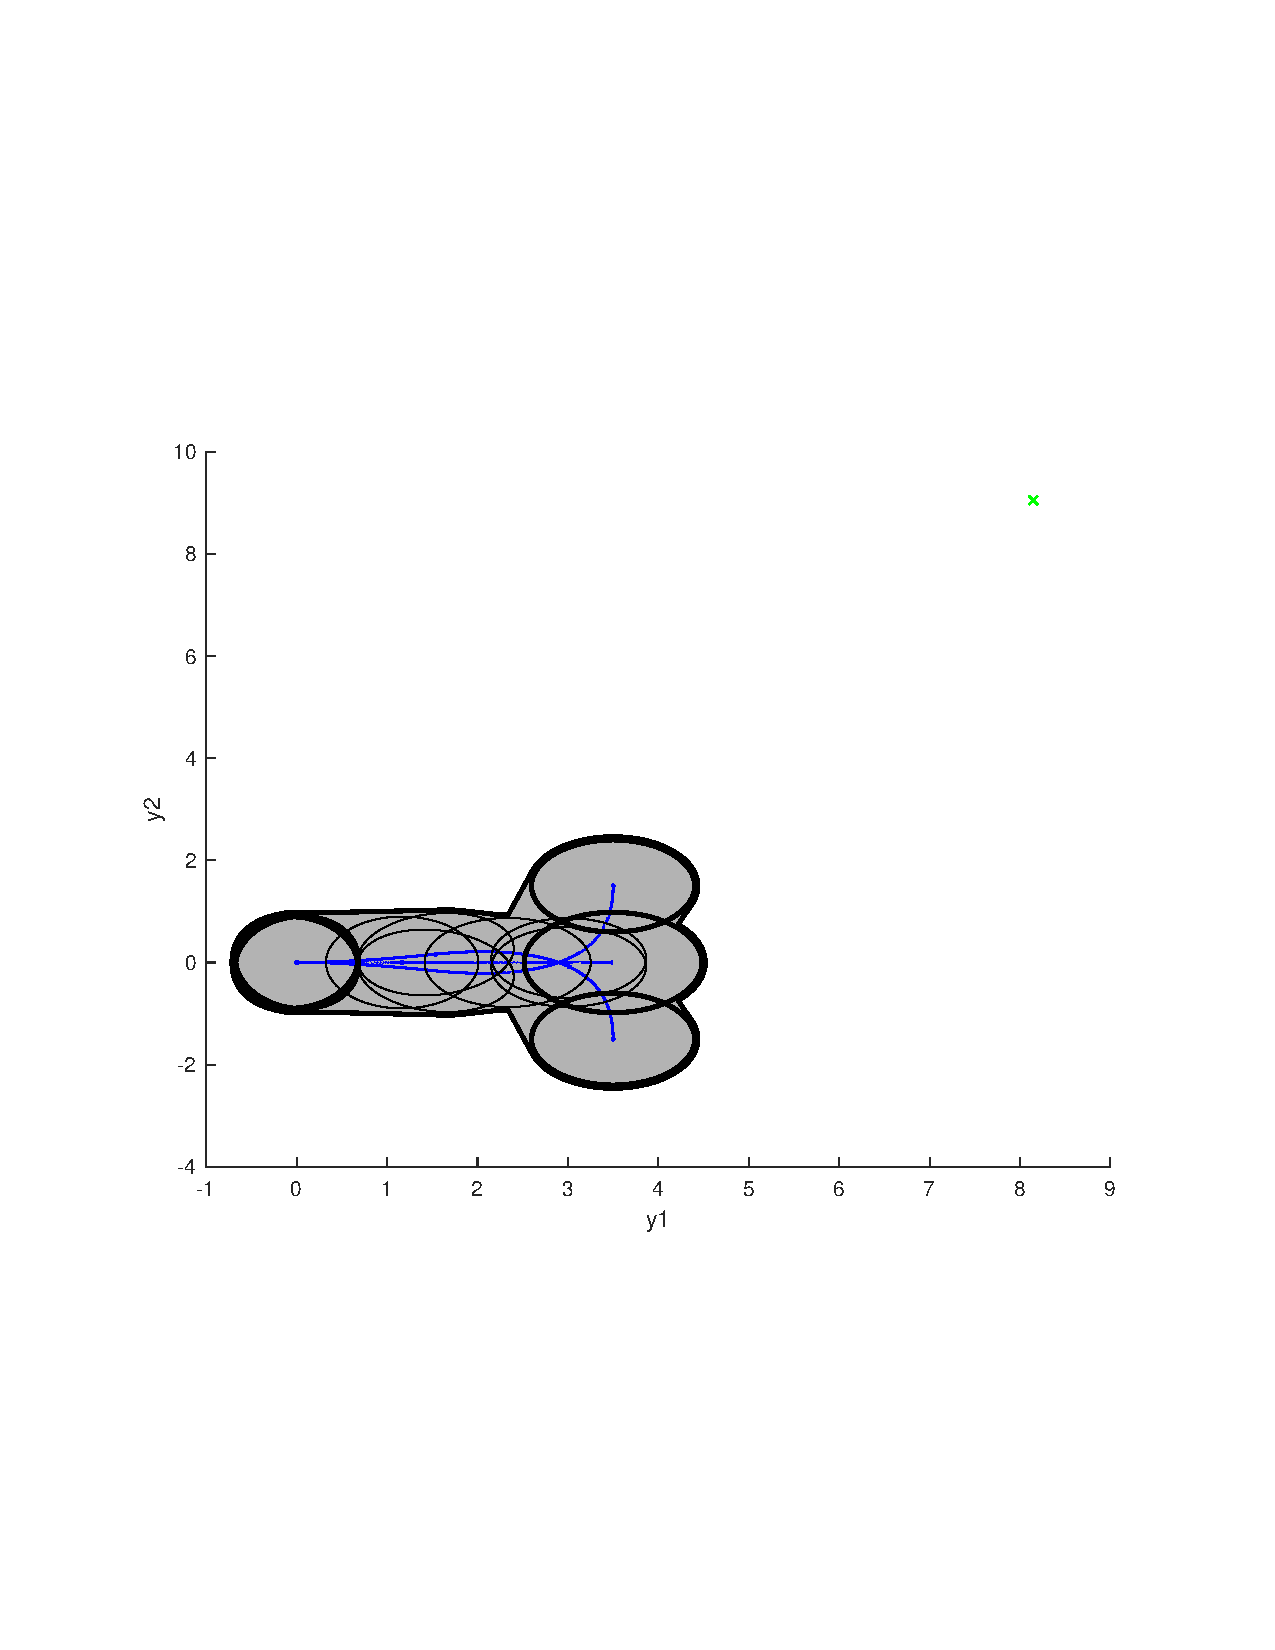
\includegraphics[scale=.5]{figures/rrtfunnel/euclidean-distance-closest-funnel1}
\caption{The three funnels in our motion primitive library, and a point in the
  state space,  selected at random, uniformly, from the interval \([0,10]\), and
  then projected down into the xy-plane.}
\end{figure}

\begin{figure}
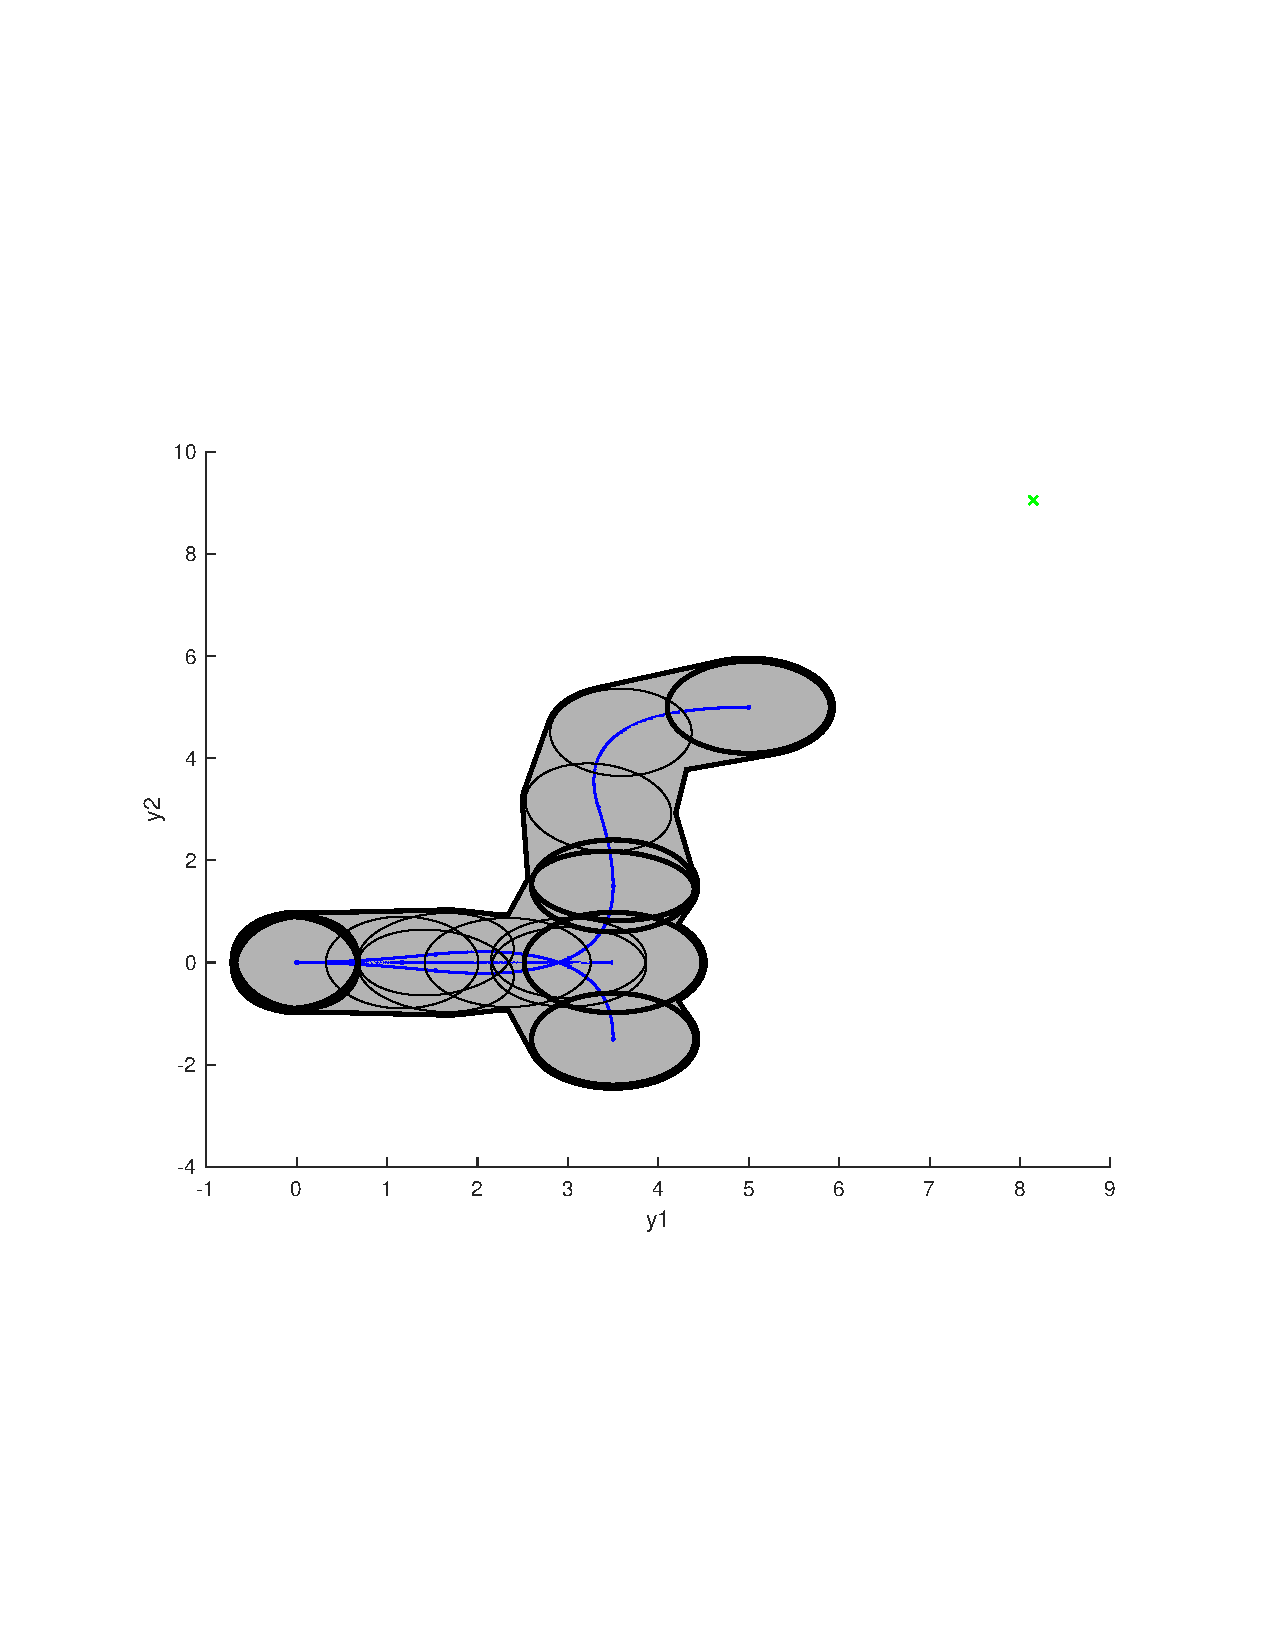
\includegraphics[scale=.5]{figures/rrtfunnel/euclidean-distance-closest-funnel2}
\caption{Tree expanded towards the point, again using the Euclidean norm as the
  metric for the local extension operator.}
\end{figure}

\begin{figure}
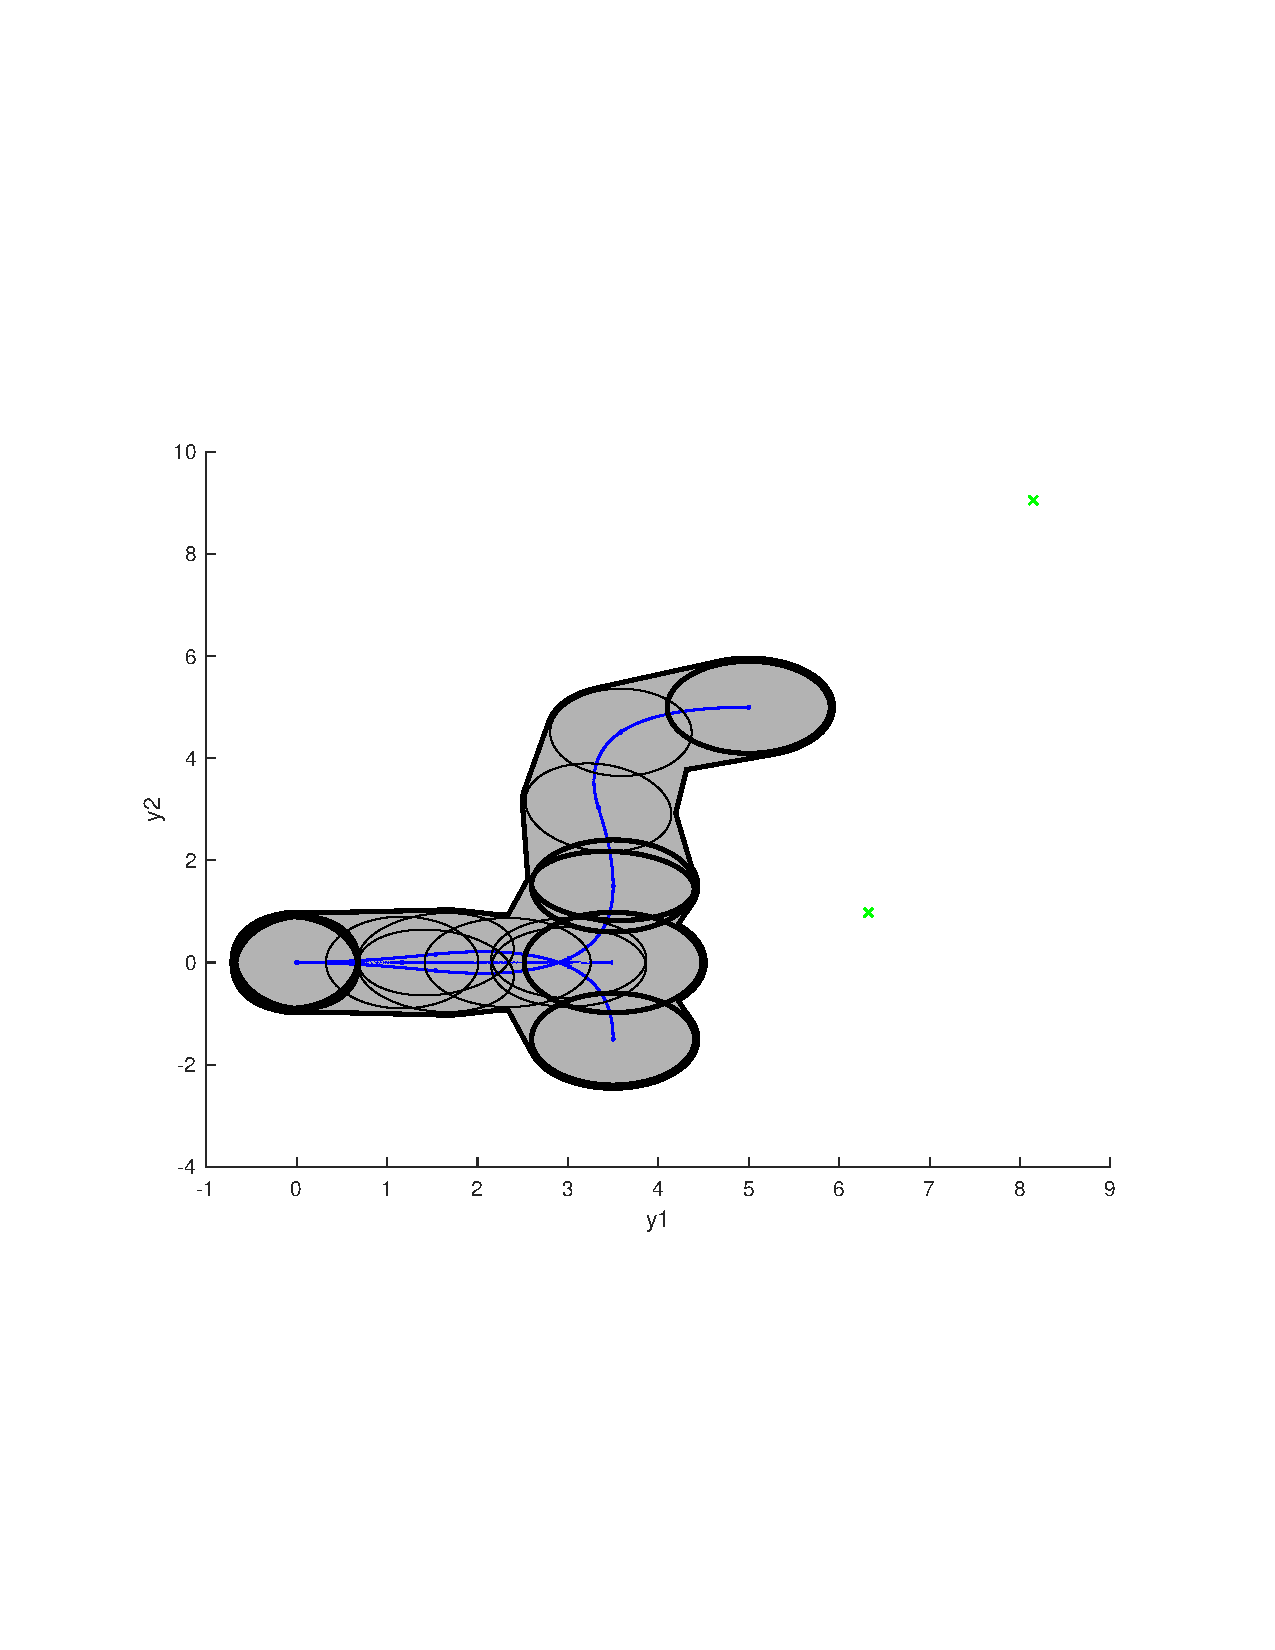
\includegraphics[scale=.5]{figures/rrtfunnel/euclidean-distance-closest-funnel3}
\caption{Another point picked uniformly from the state space.}
\end{figure}

\begin{figure}
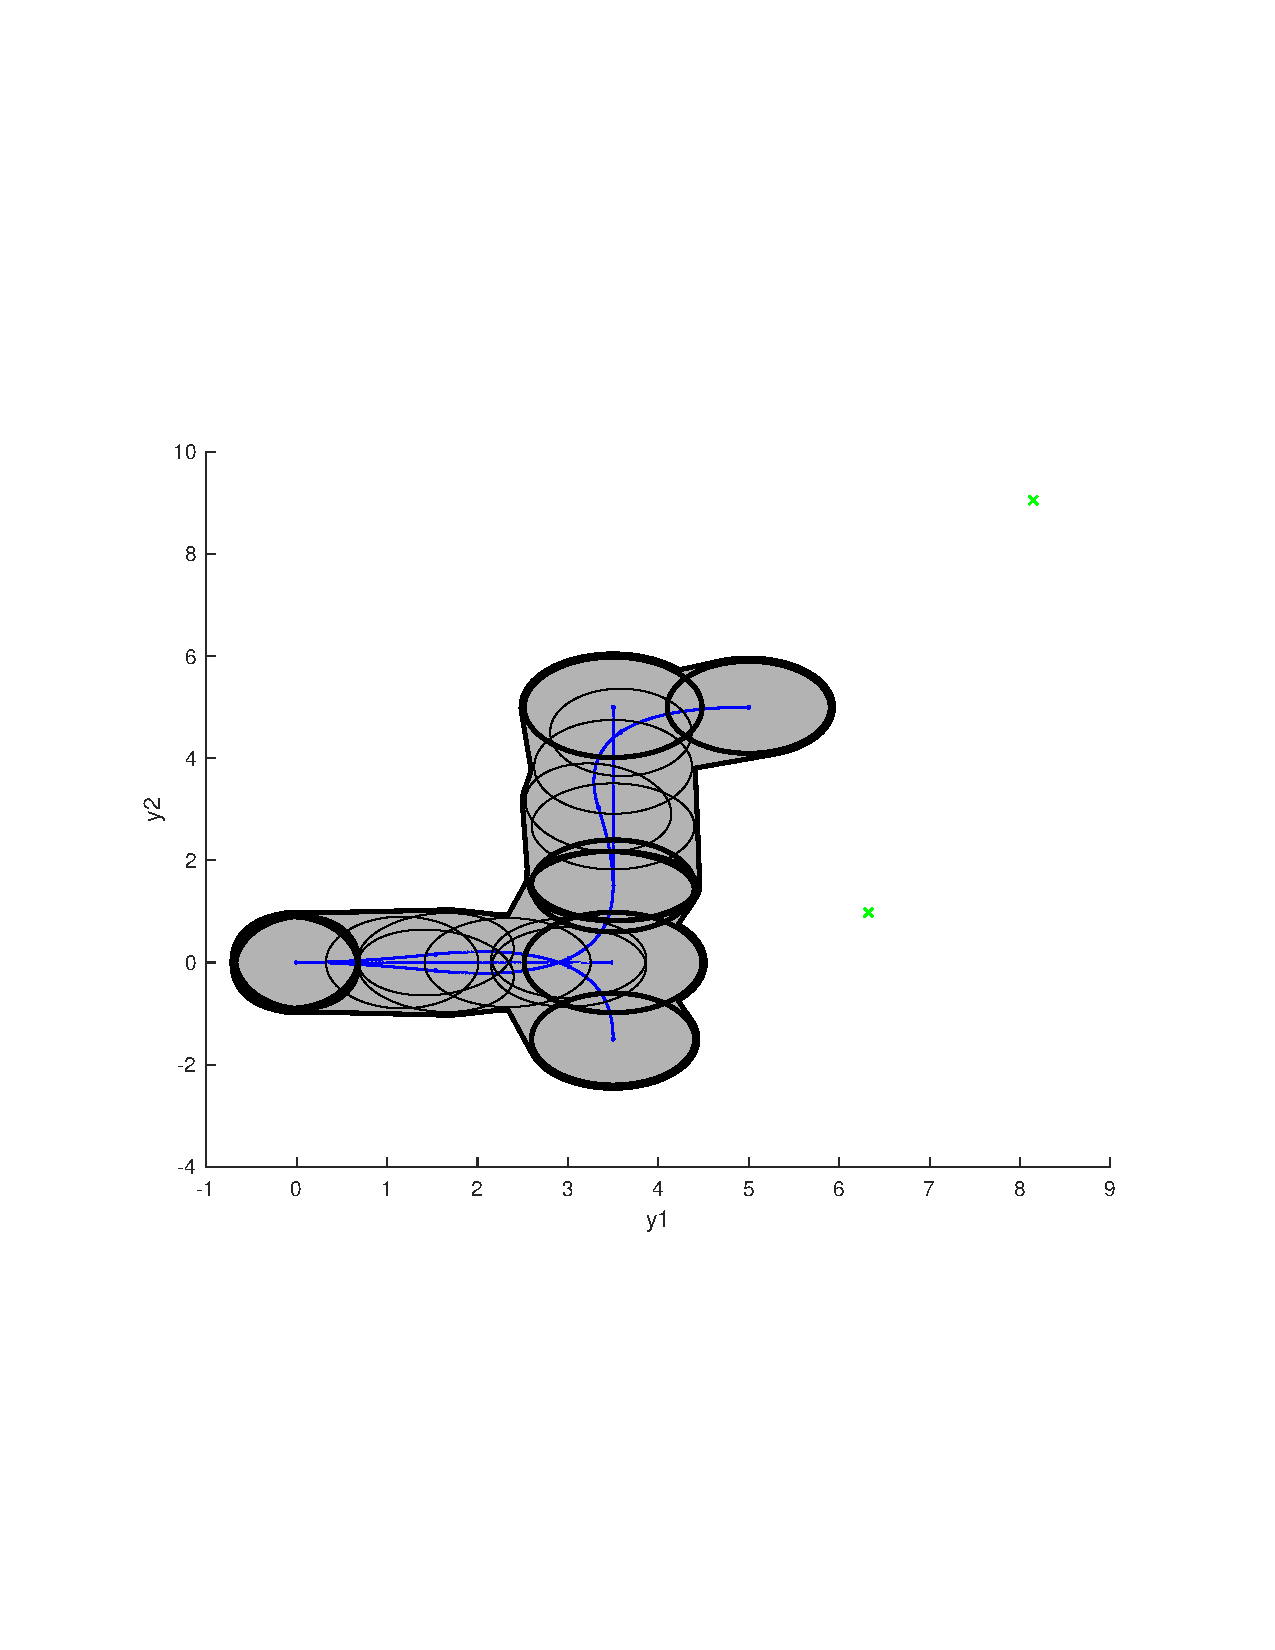
\includegraphics[scale=.5]{figures/rrtfunnel/euclidean-distance-closest-funnel4}
\caption{The funnel chosen by the local extension operator shows the limitations
of the Euclidean distance metric in the RRTFunnel algorithm.}
\end{figure}

This weakness is not unexpected if you take into consideration the non-holonomic
dynamics of our model vehicle. Thus the \textit{Euclidean metric} is a poor
measure of the cost-to-go of the system
\ref{non-holonomic-vehicle-euclidean-weakness}. This is not unexpected as
the \textit{Euclidean metric} is only a proper metric for holonomic vehicles \cite{parkFeedbackMotionPlanning2015}.
(TODO -show this!).


\begin{figure}
  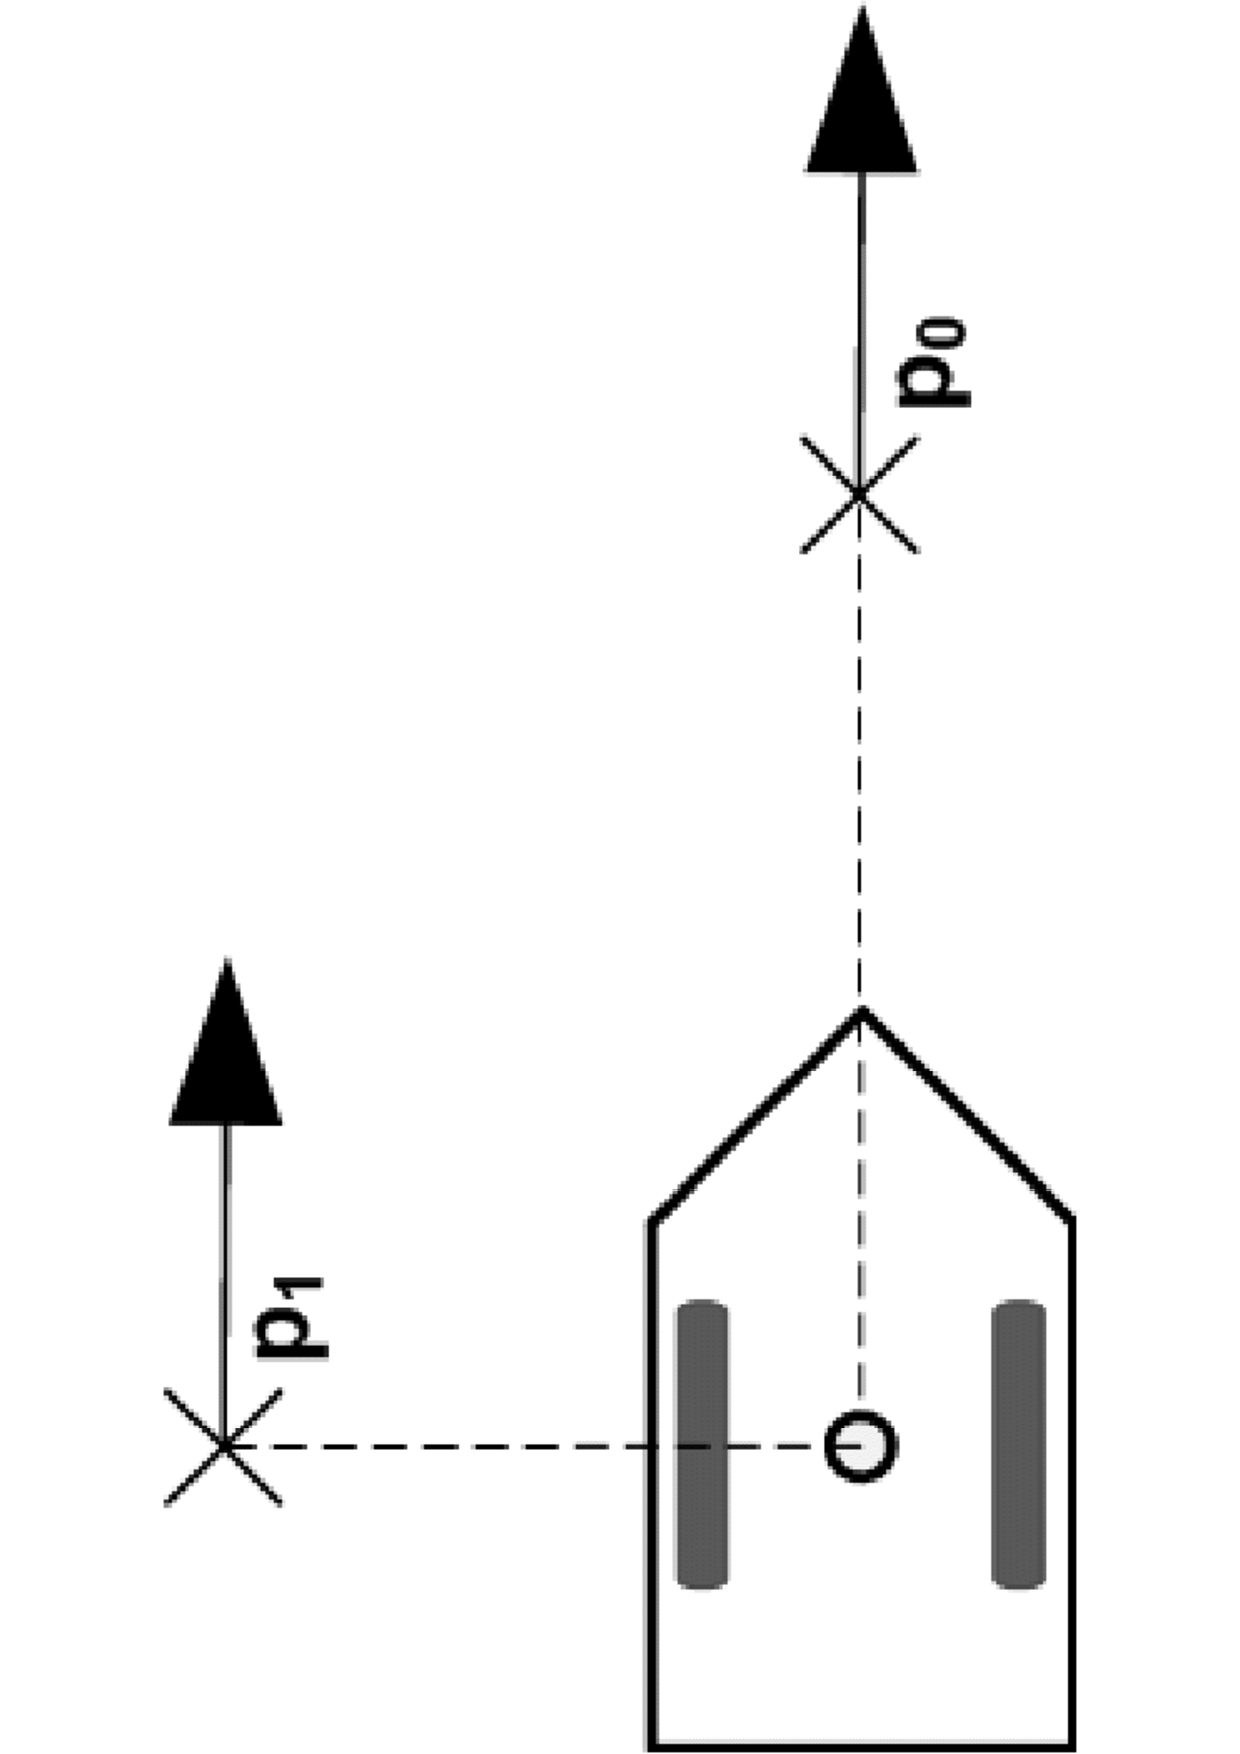
\includegraphics[scale=.3,angle=-90]{figures/rrtfunnel/non-holonomic-vehicle-euclidean-weakness}
  \caption{Consider two poses \(p_0\) and \(p_1\). Although \(p_1\) is nearer
    the robot in Euclidean distance it is harder to get to due to differential
    constraints. In this paper, we propose a directed distance function
    applicable to unicycle- type vehicles, that properly reflects the true
    cost-to-go of the system under the non-holonomic constraint. (figure
    courtesy of \cite{parkFeedbackMotionPlanning2015})}
\label{fig:non-holonomic-vehicle-euclidean-weakness}
\end{figure}

A look at the growth of the tree in the uniform sampling space \([-50,50]\) for
\(x\) and \(y\), and \([0,pi]\) for \(\theta\), and \[[0,10]\] for
\(\dot{\theta}\), gives:

\begin{figure}
  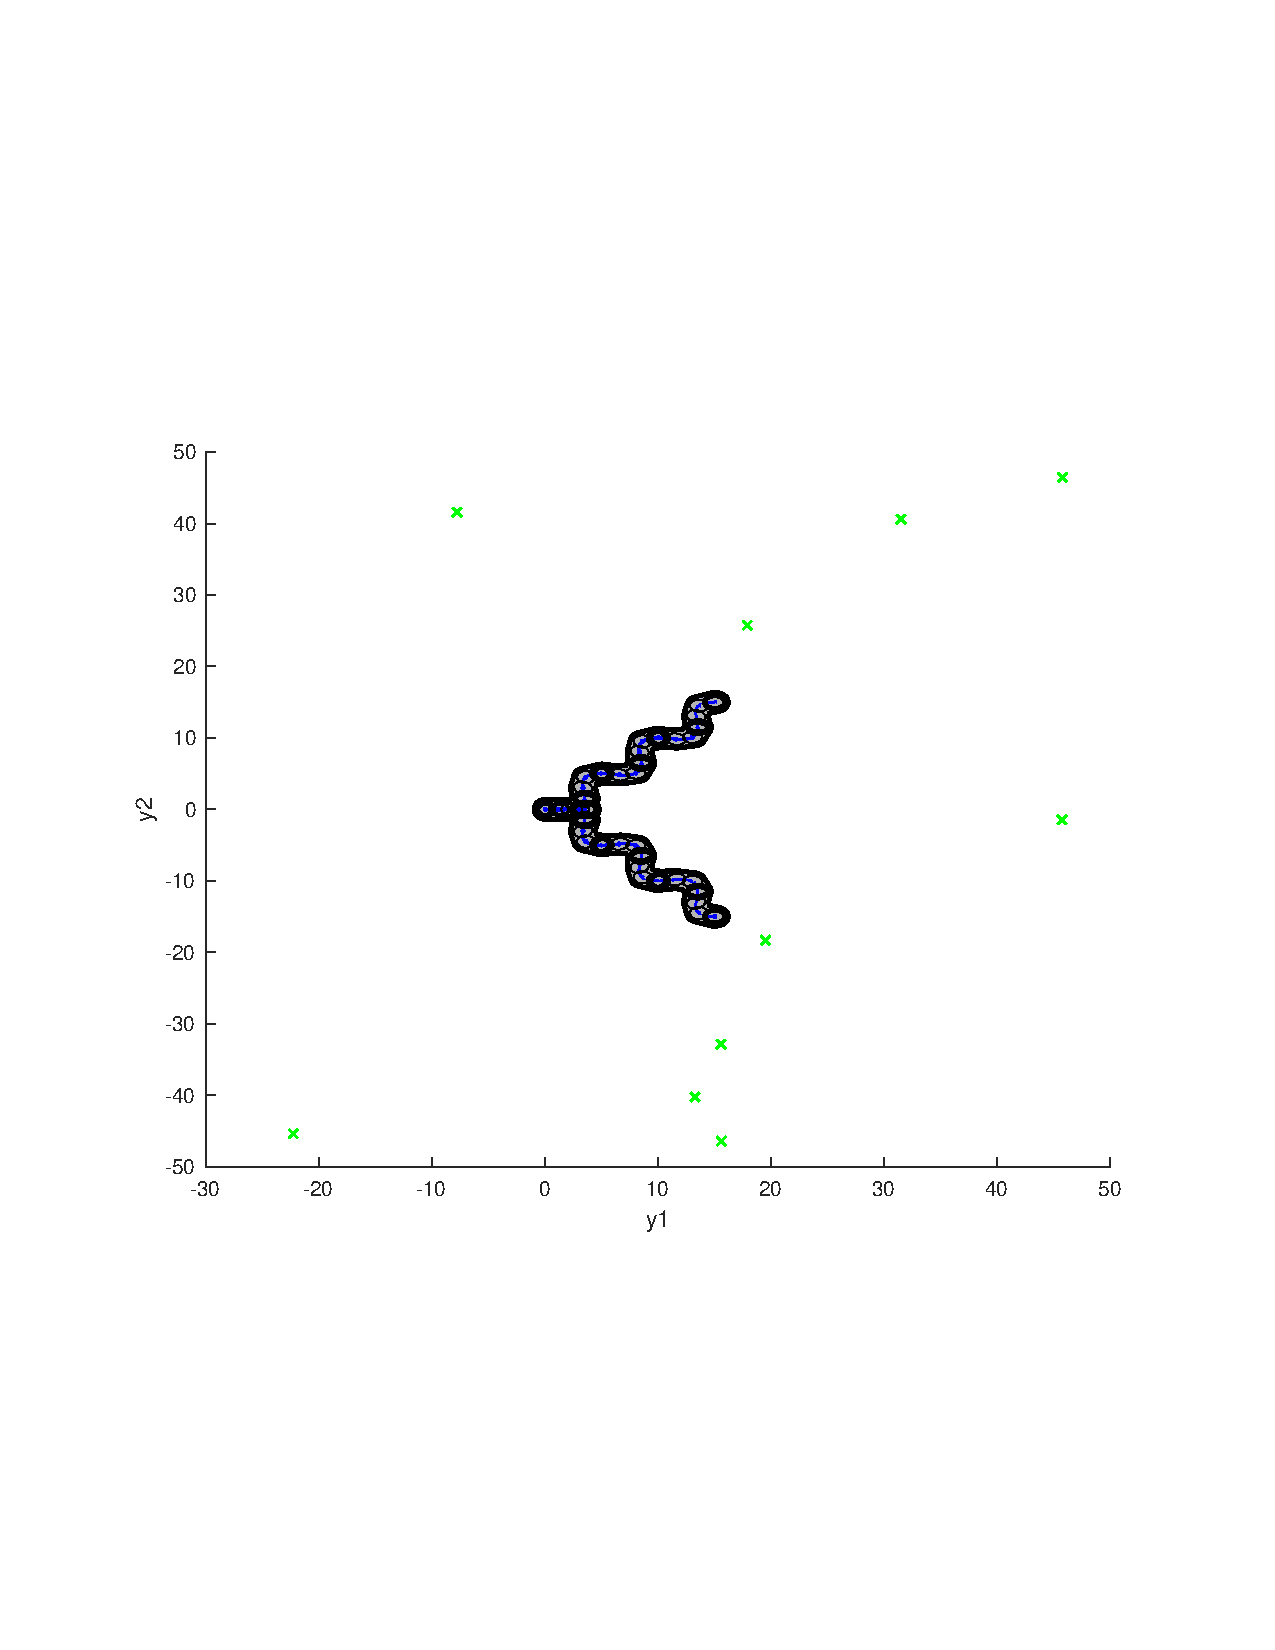
\includegraphics[scale=.5]{figures/rrtfunnel/rrtfunnel-10samples}
  \caption{The growth of the \textit{RRTFunnel} tree with three motion
    primitives, uniform sampling and the standard euclidean distance metric
    after 10 samples.}
\end{figure}

\begin{figure}
  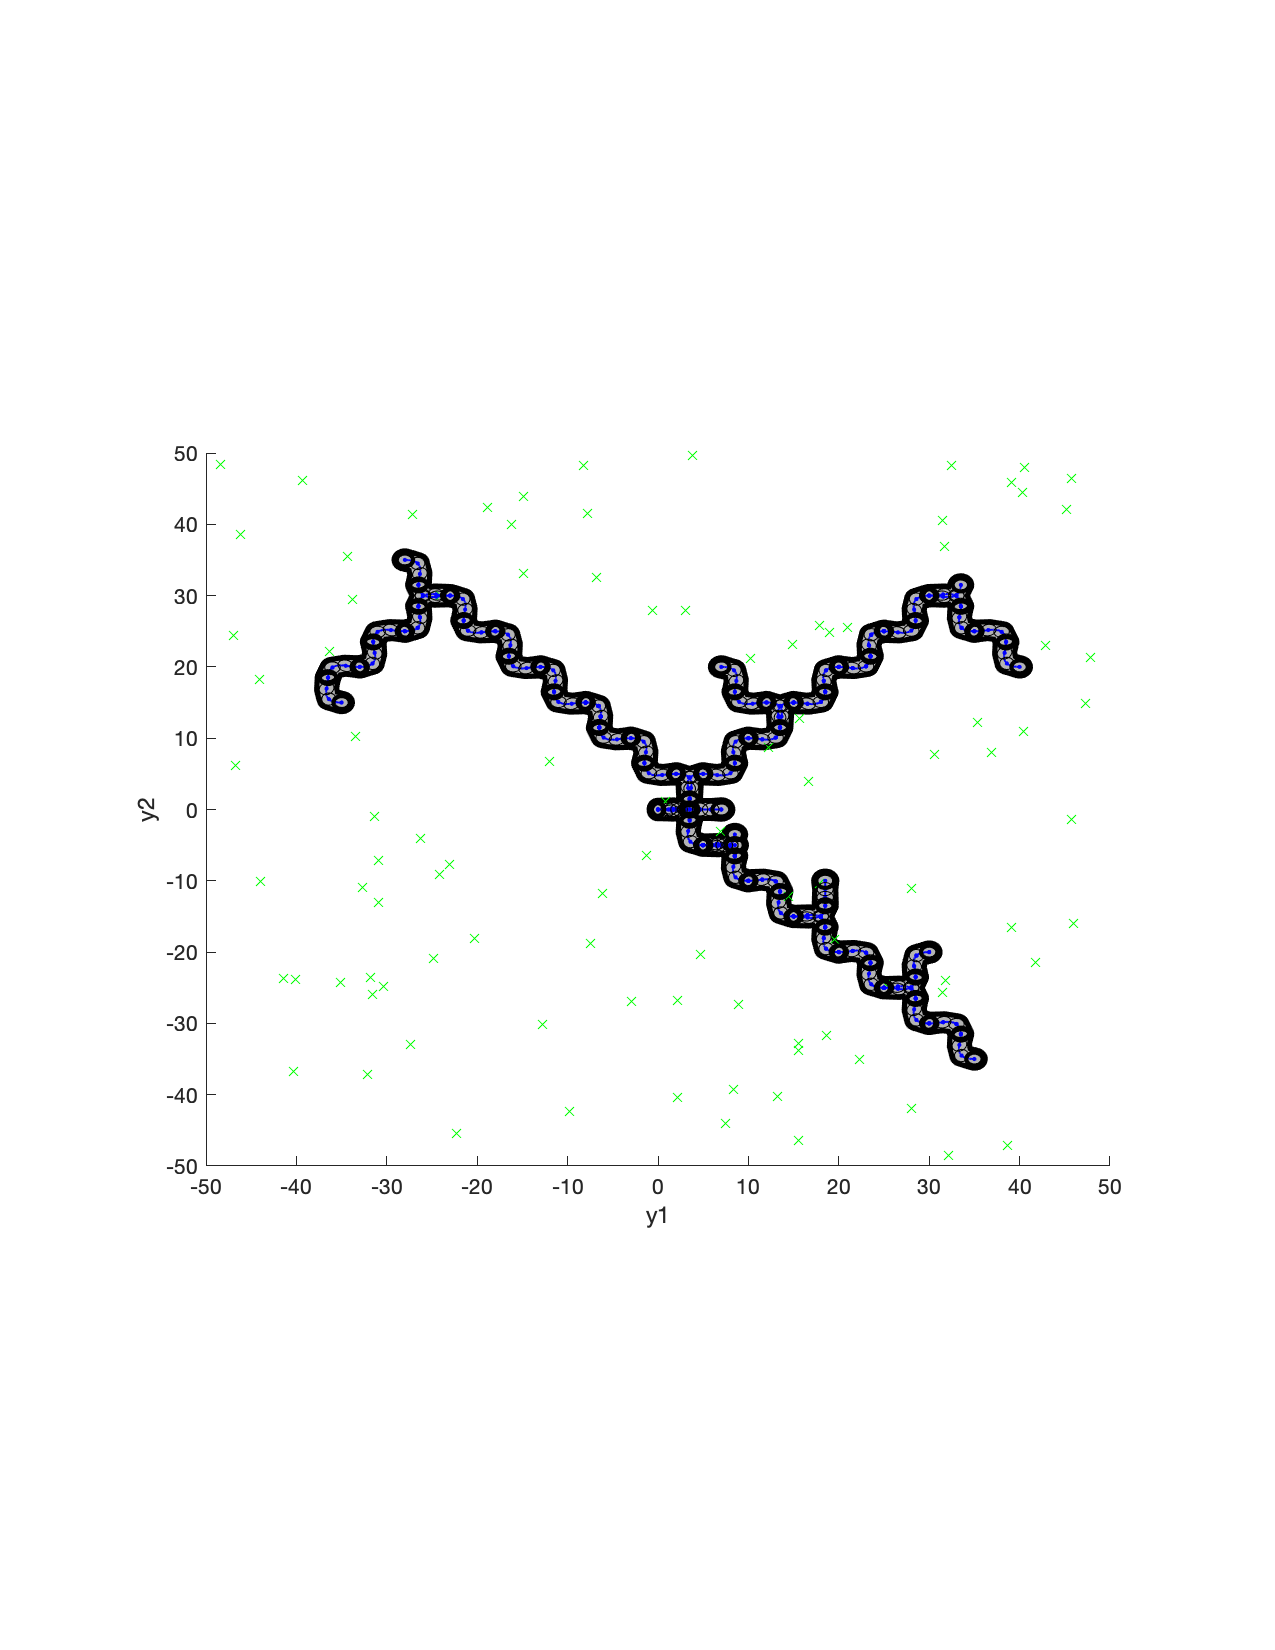
\includegraphics[scale=.5]{figures/rrtfunnel/rrtfunnel-100samples}
  \caption{The growth of the \textit{RRTFunnel} tree with three motion
    primitives, uniform sampling and the standard euclidean distance metric
    after 100 samples. The tree grows quickly into unexplored areas of the
    space, like expected.}
\end{figure}


\begin{figure}
  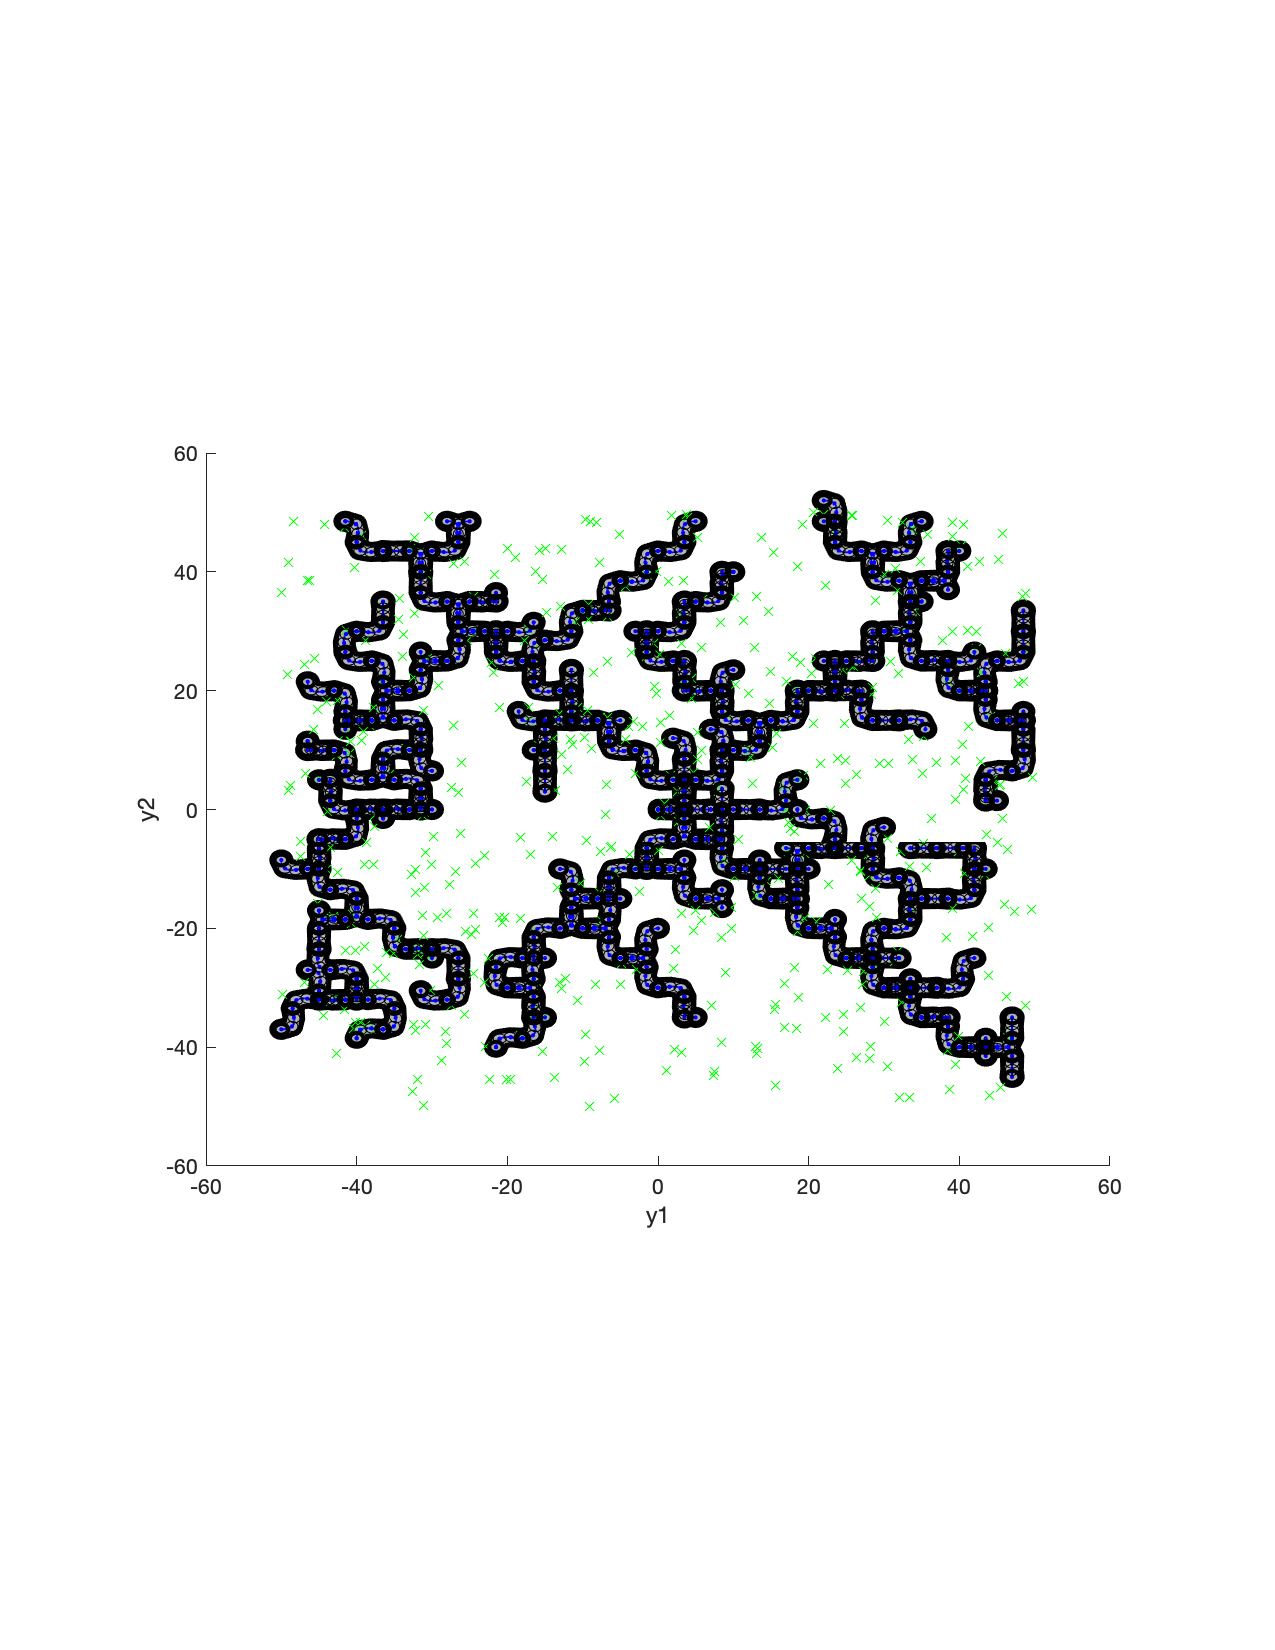
\includegraphics[scale=.5]{figures/rrtfunnel/rrtfunnel-500samples}
  \caption{The growth of the \textit{RRTFunnel} tree with three motion
    primitives, uniform sampling and the standard euclidean distance metric
    after 500 samples.}
\end{figure}


\begin{figure}
  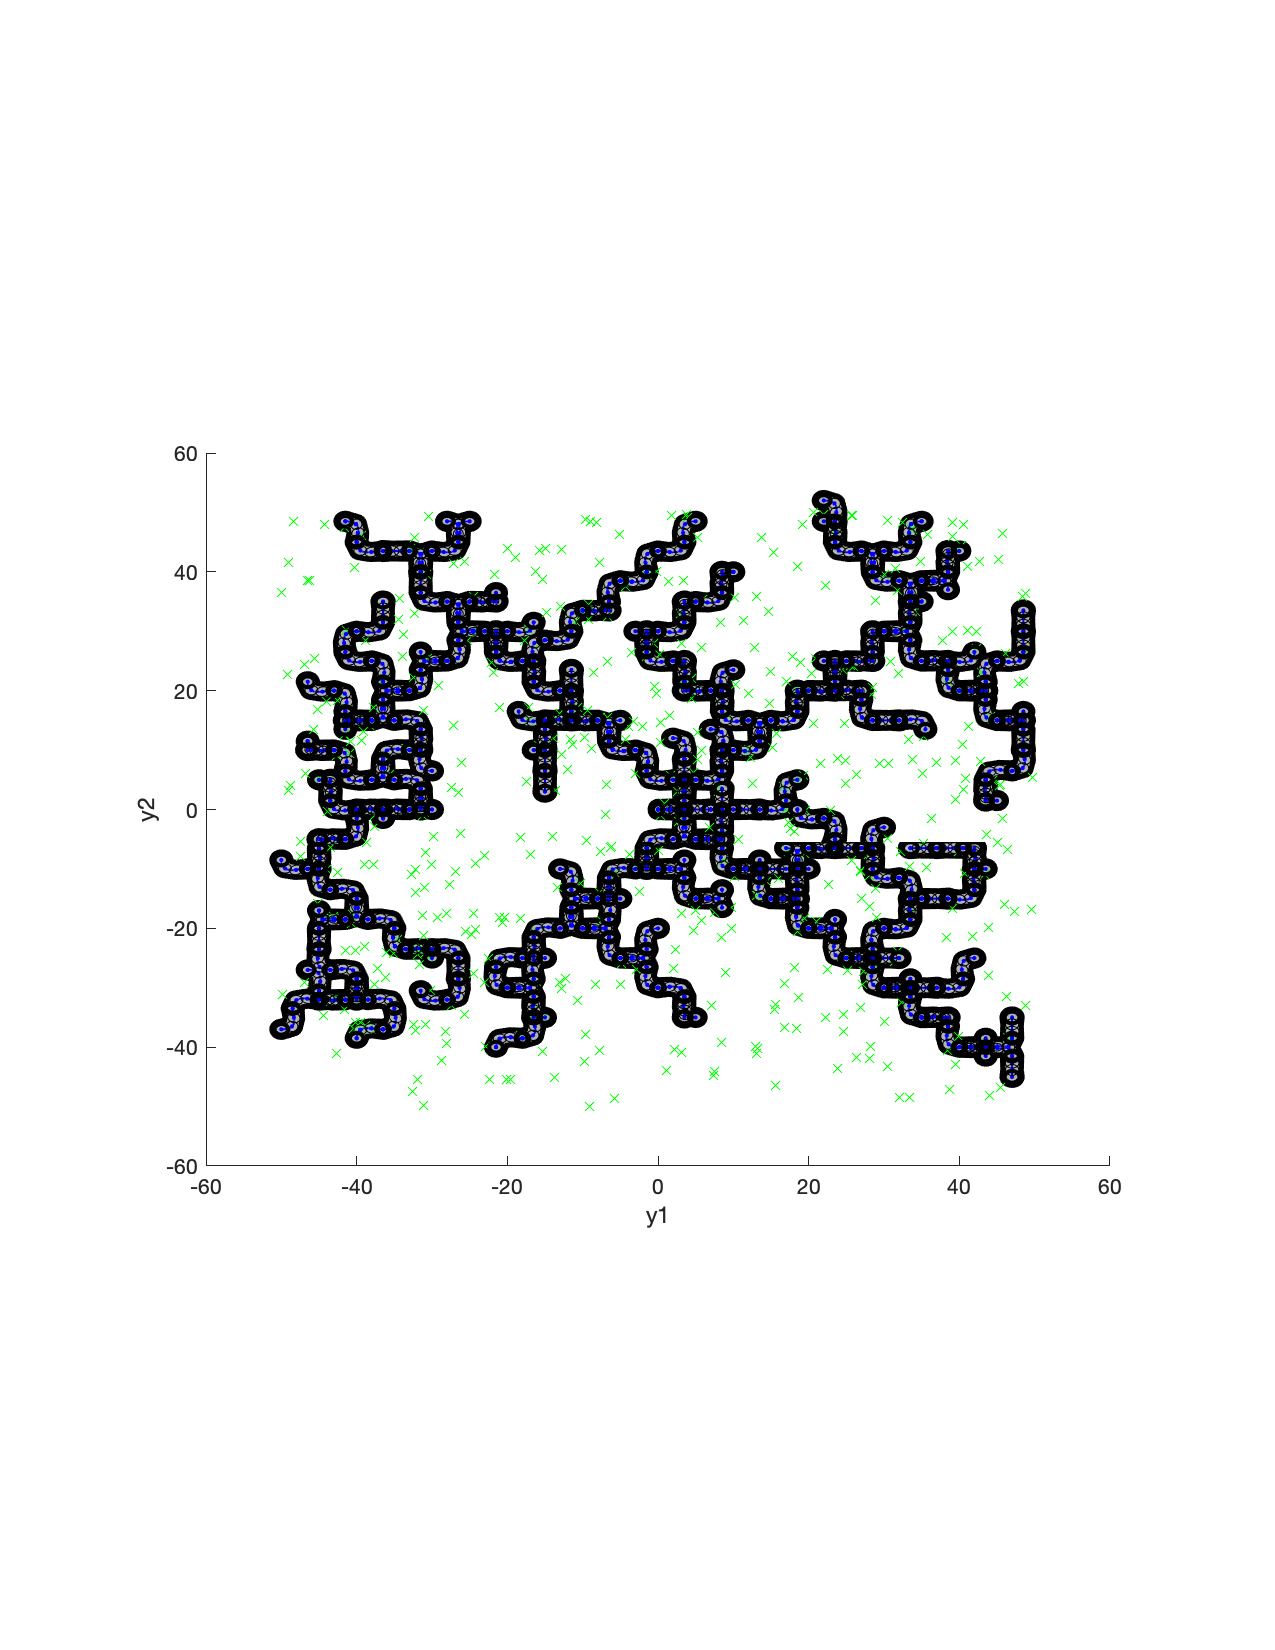
\includegraphics[scale=.5]{figures/rrtfunnel/rrtfunnel-500samples}
  \caption{The growth of the \textit{RRTFunnel} tree with three motion
    primitives, uniform sampling and the standard euclidean distance metric
    after 1000 samples.}
\end{figure}

\subsection{Modified Euclidean distance metric}

One of the problems of the euclidean metric is that is is oblivious to the
heading of the car. If the metric considered the heading only as an issue in the
case that the point is close, in the sense of Euclidean distance in the plane,
and started worrying about the heading as it got closer, a metric which weights
the angle \(\theta\) in the distance metric can be considered, thus let:
\begin{align}
  d(x_1,x_2) &= \sqrt(x^2 + y^2 + f(x^2 + y^2)*\theta) \\
  f(a) = \frac{1}{a}
\end{align}

\begin{figure}
  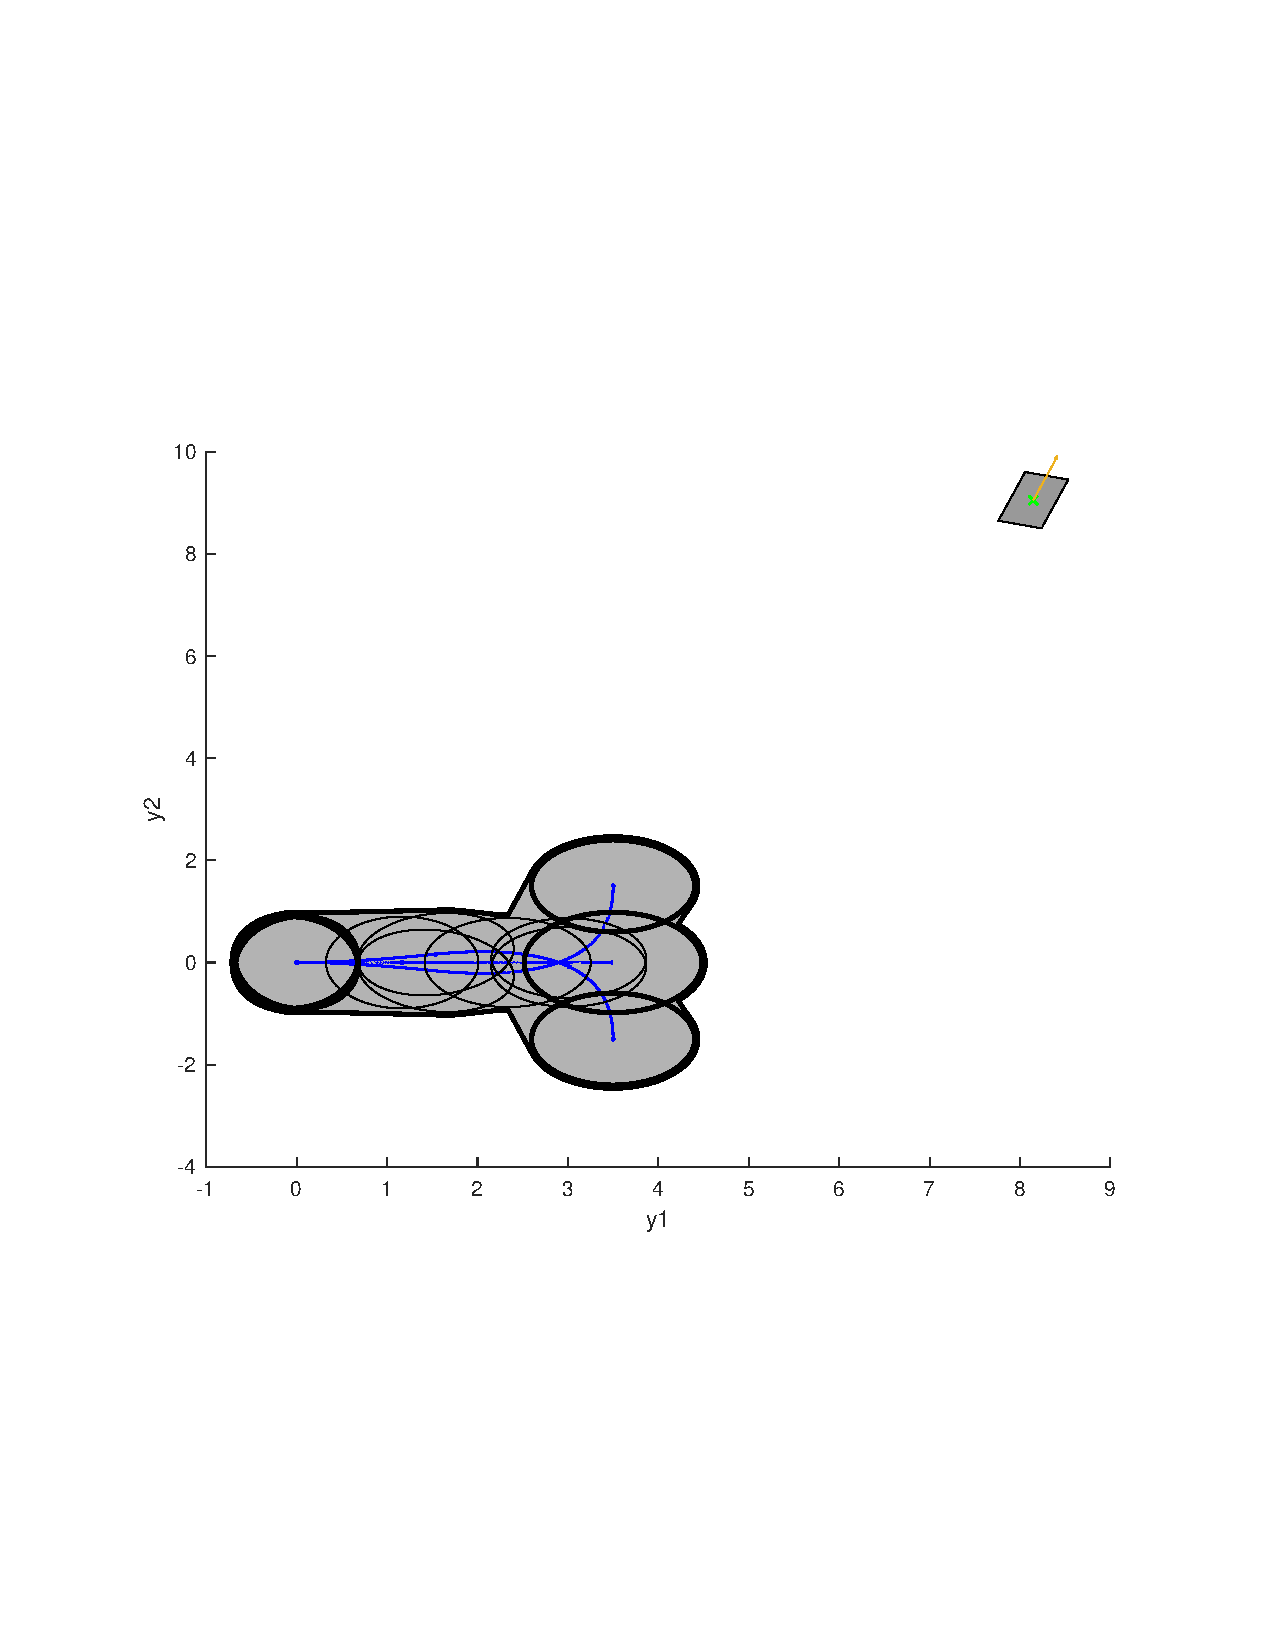
\includegraphics[scale=.5]{figures/rrtfunnel/modified-euclidean-distance-closest-funnel1}
  \caption{Car in state space picked at random from a uniform distribution on
    the interval \([0,10]\), for \(x\) and \(y\), and \([0,2\pi)\) for \(\theta\).}
\end{figure}

\begin{figure}
  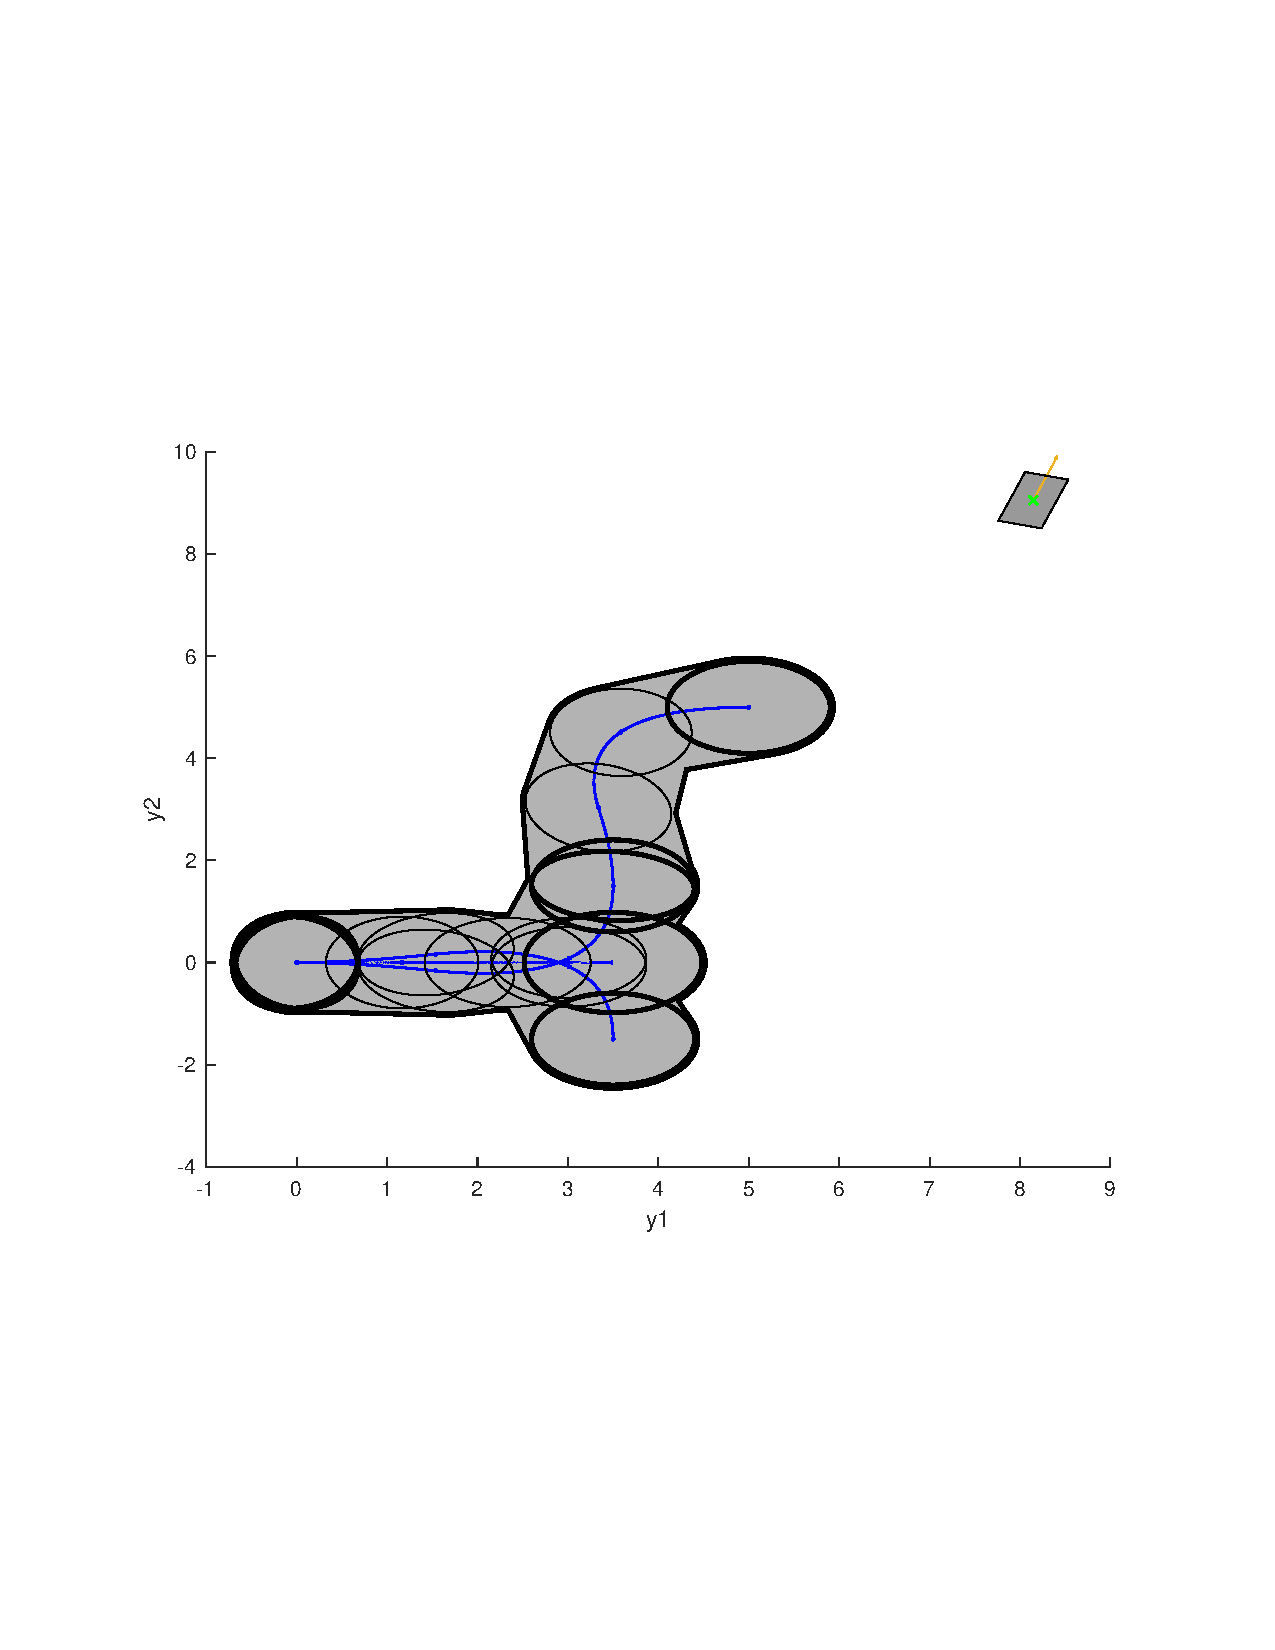
\includegraphics[scale=.5]{figures/rrtfunnel/modified-euclidean-distance-closest-funnel2}
  \caption{The closest funnel picked was left, and the expand operation picked
    the right funnel to extend the tree towards the point picked, like expected,
  and the same behaviour shown in the normal \textit{euclidean distance metric}.}
\end{figure}


\begin{figure}
  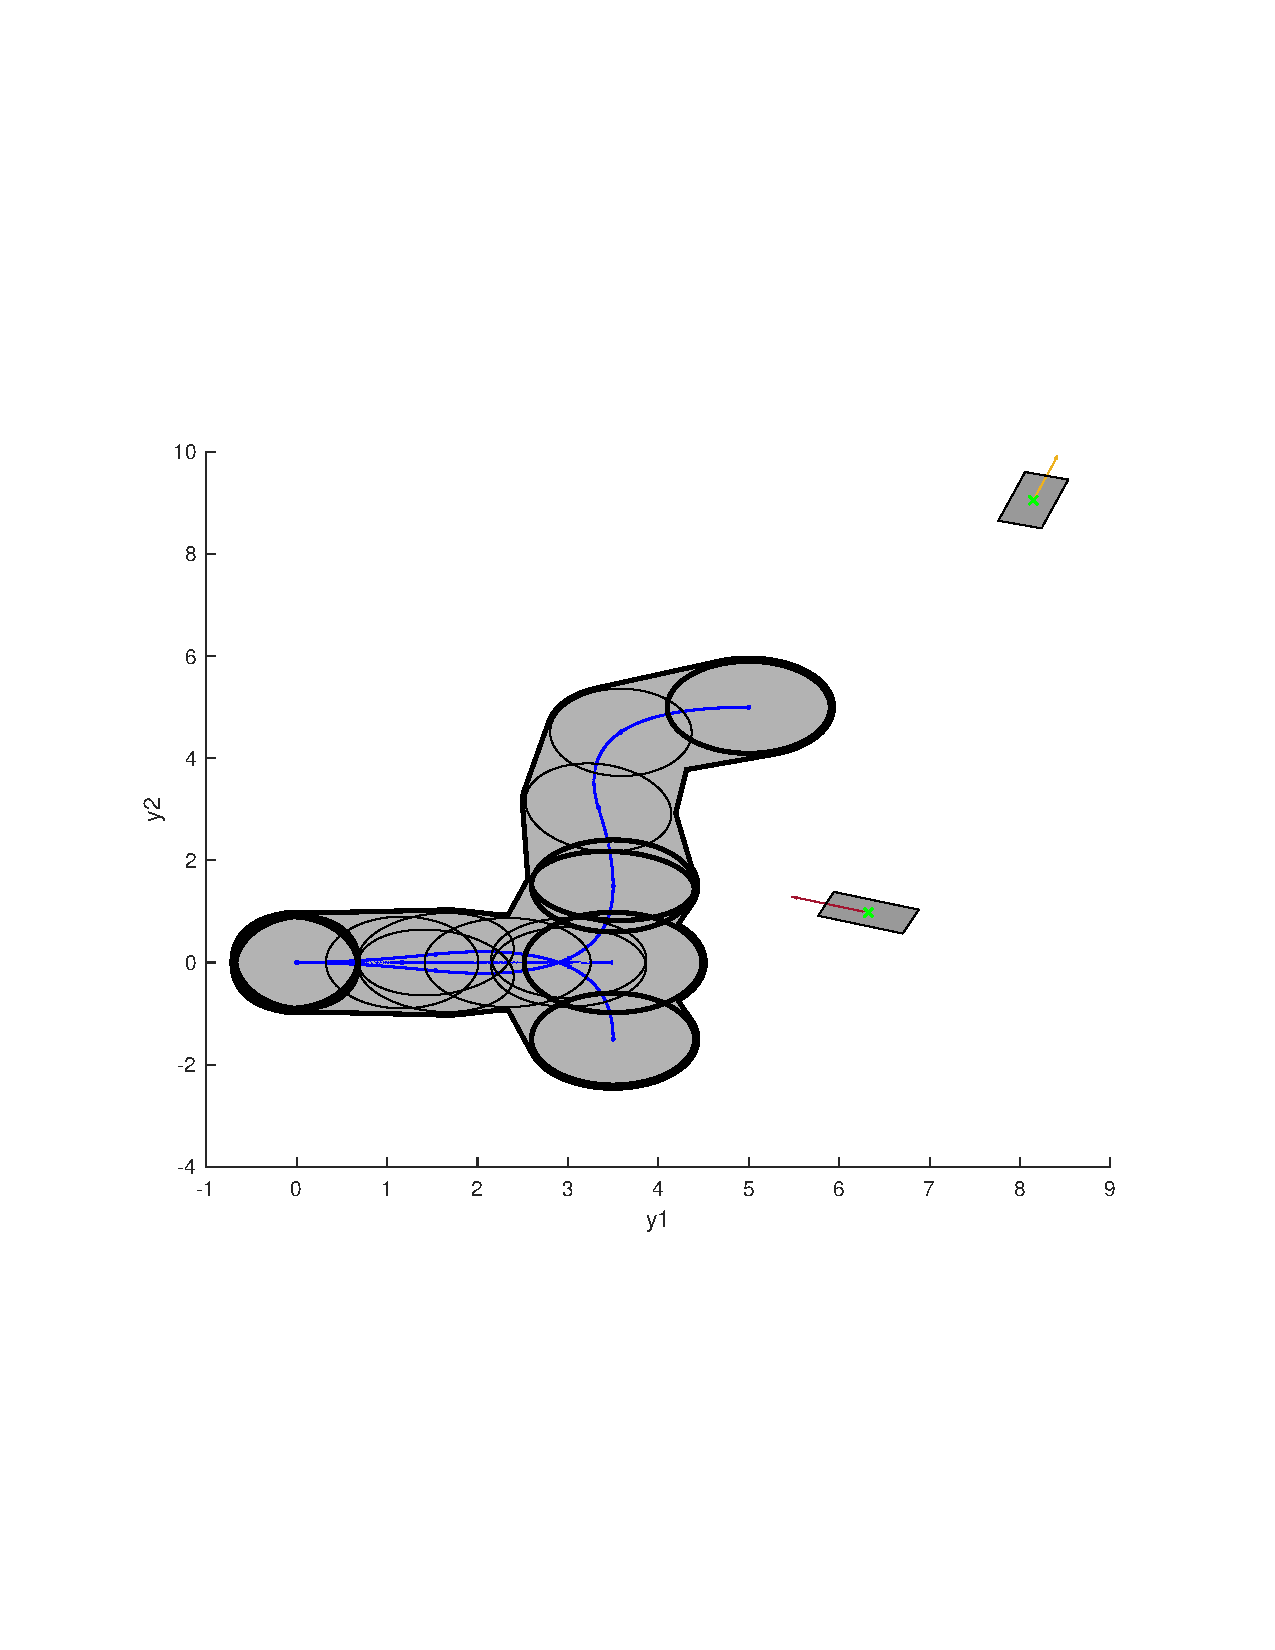
\includegraphics[scale=.5]{figures/rrtfunnel/modified-euclidean-distance-closest-funnel3}
  \caption{Another car state picked at random.}
\end{figure}

\begin{figure}
  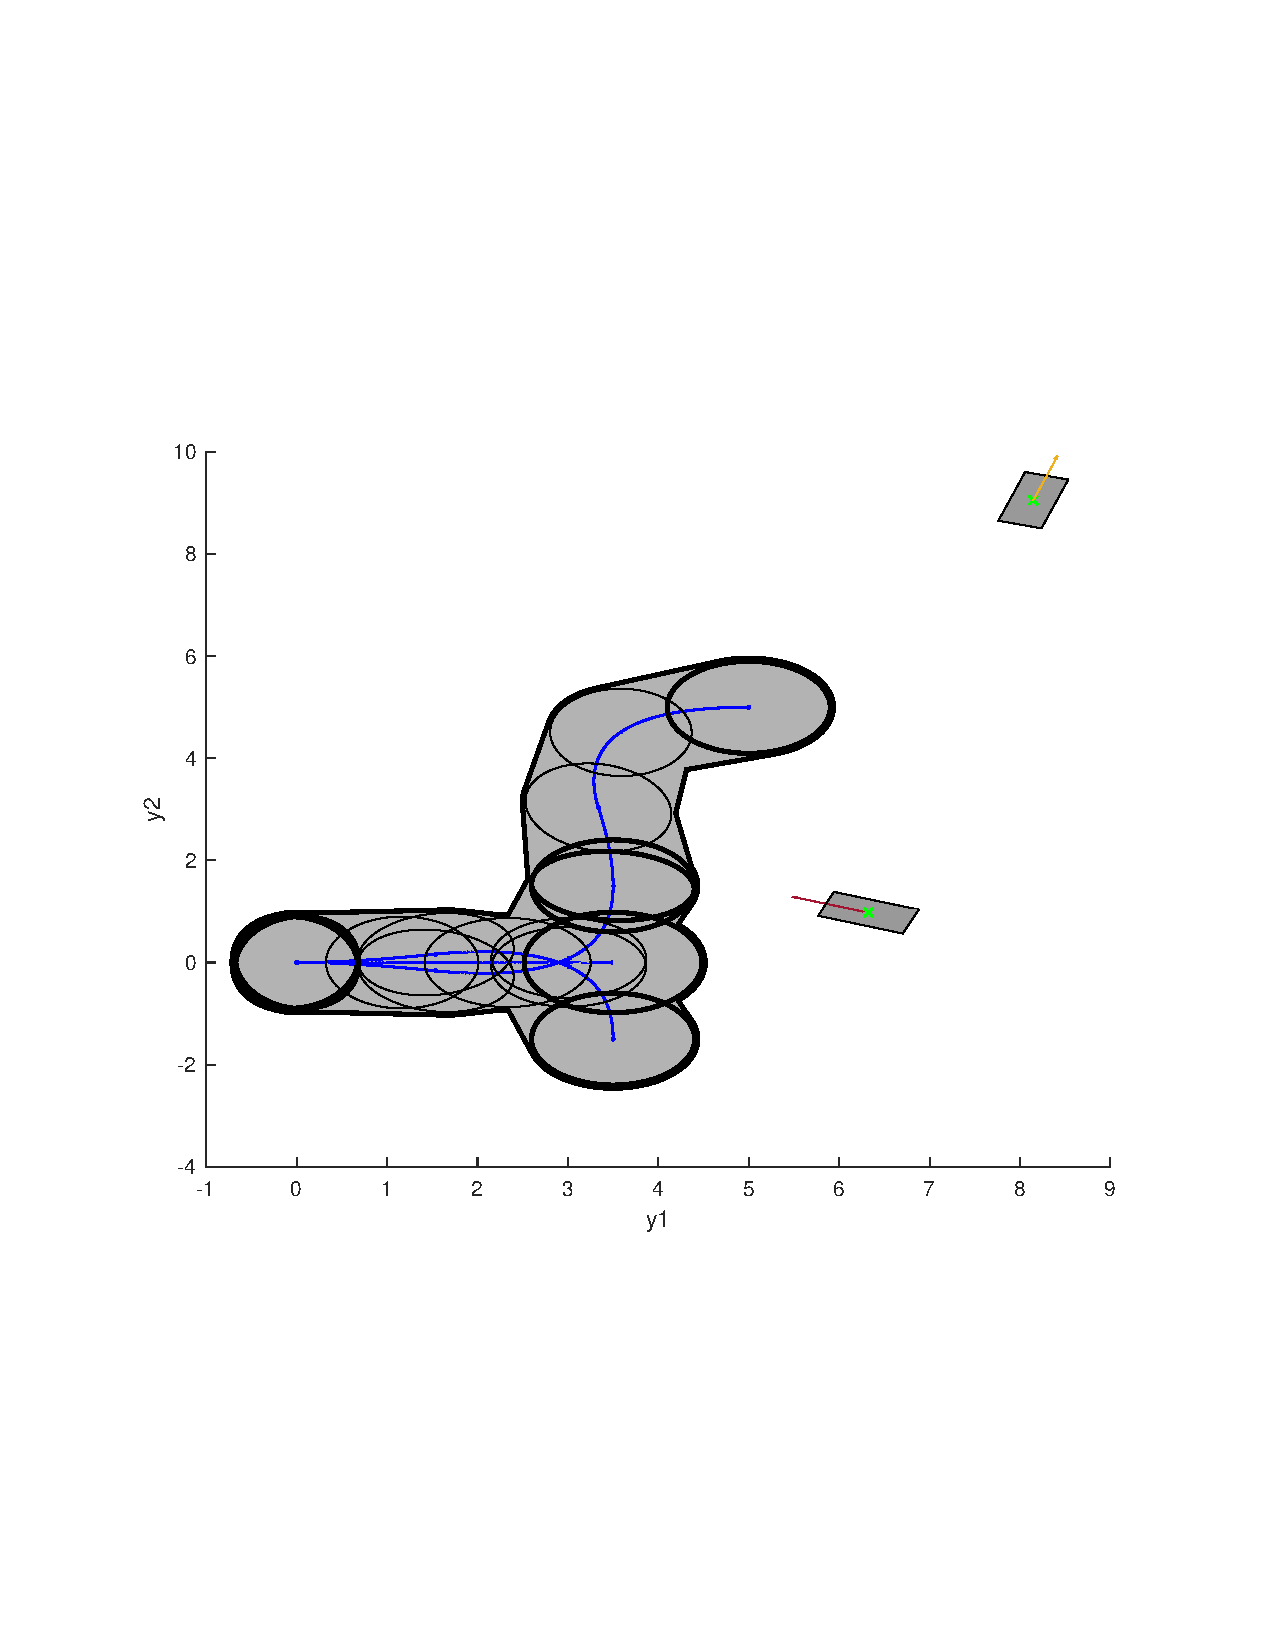
\includegraphics[scale=.5]{figures/rrtfunnel/modified-euclidean-distance-closest-funnel4}
  \caption{This time the extent operator chose the same funnel as in the
    previous operation. Is this how we want our extension operator to work? can
    they overlap?}
\end{figure}


\begin{figure}
  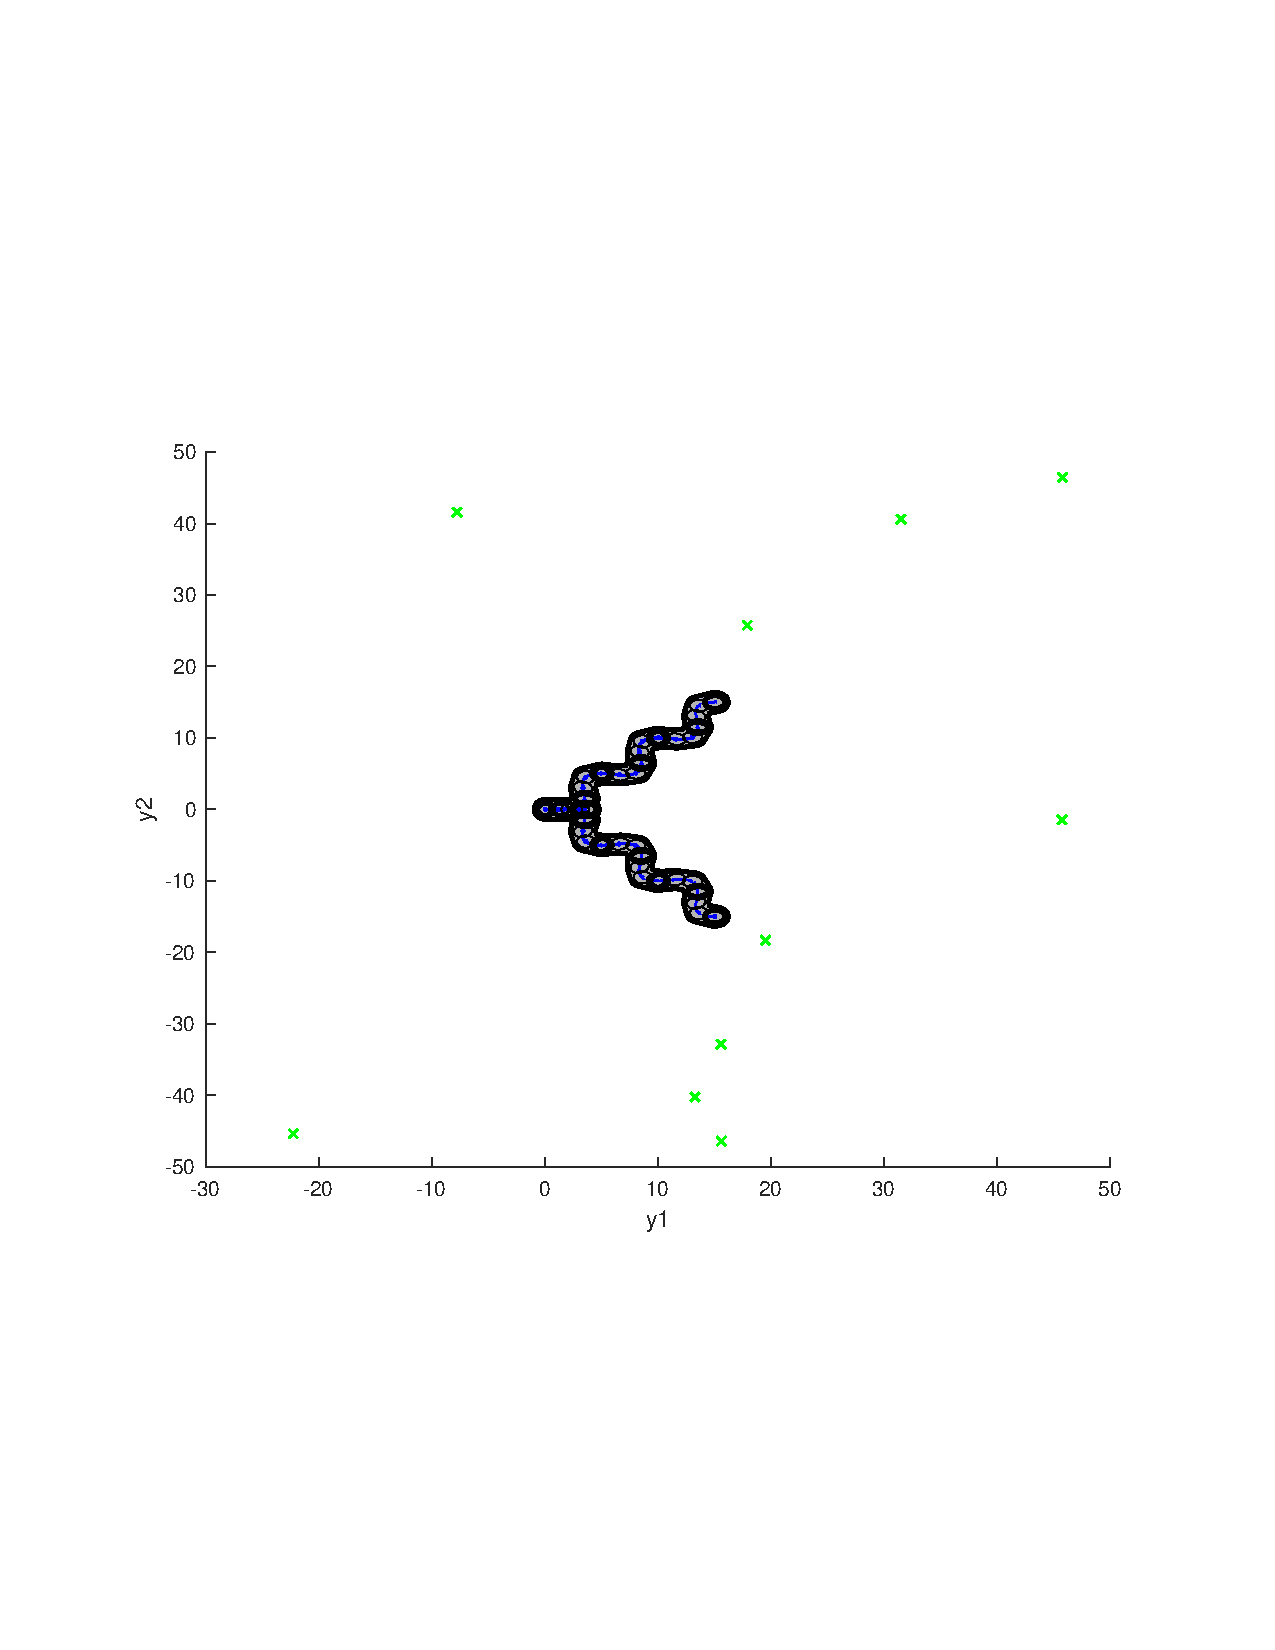
\includegraphics[scale=.5]{figures/rrtfunnel/rrtfunnel-modified-euclidean-10samples}
  \caption{The growth of the \textit{RRTFunnel} tree with three motion
    primitives, uniform sampling and the modified euclidean distance metric
    after 10 samples.}
\end{figure}

\begin{figure}
  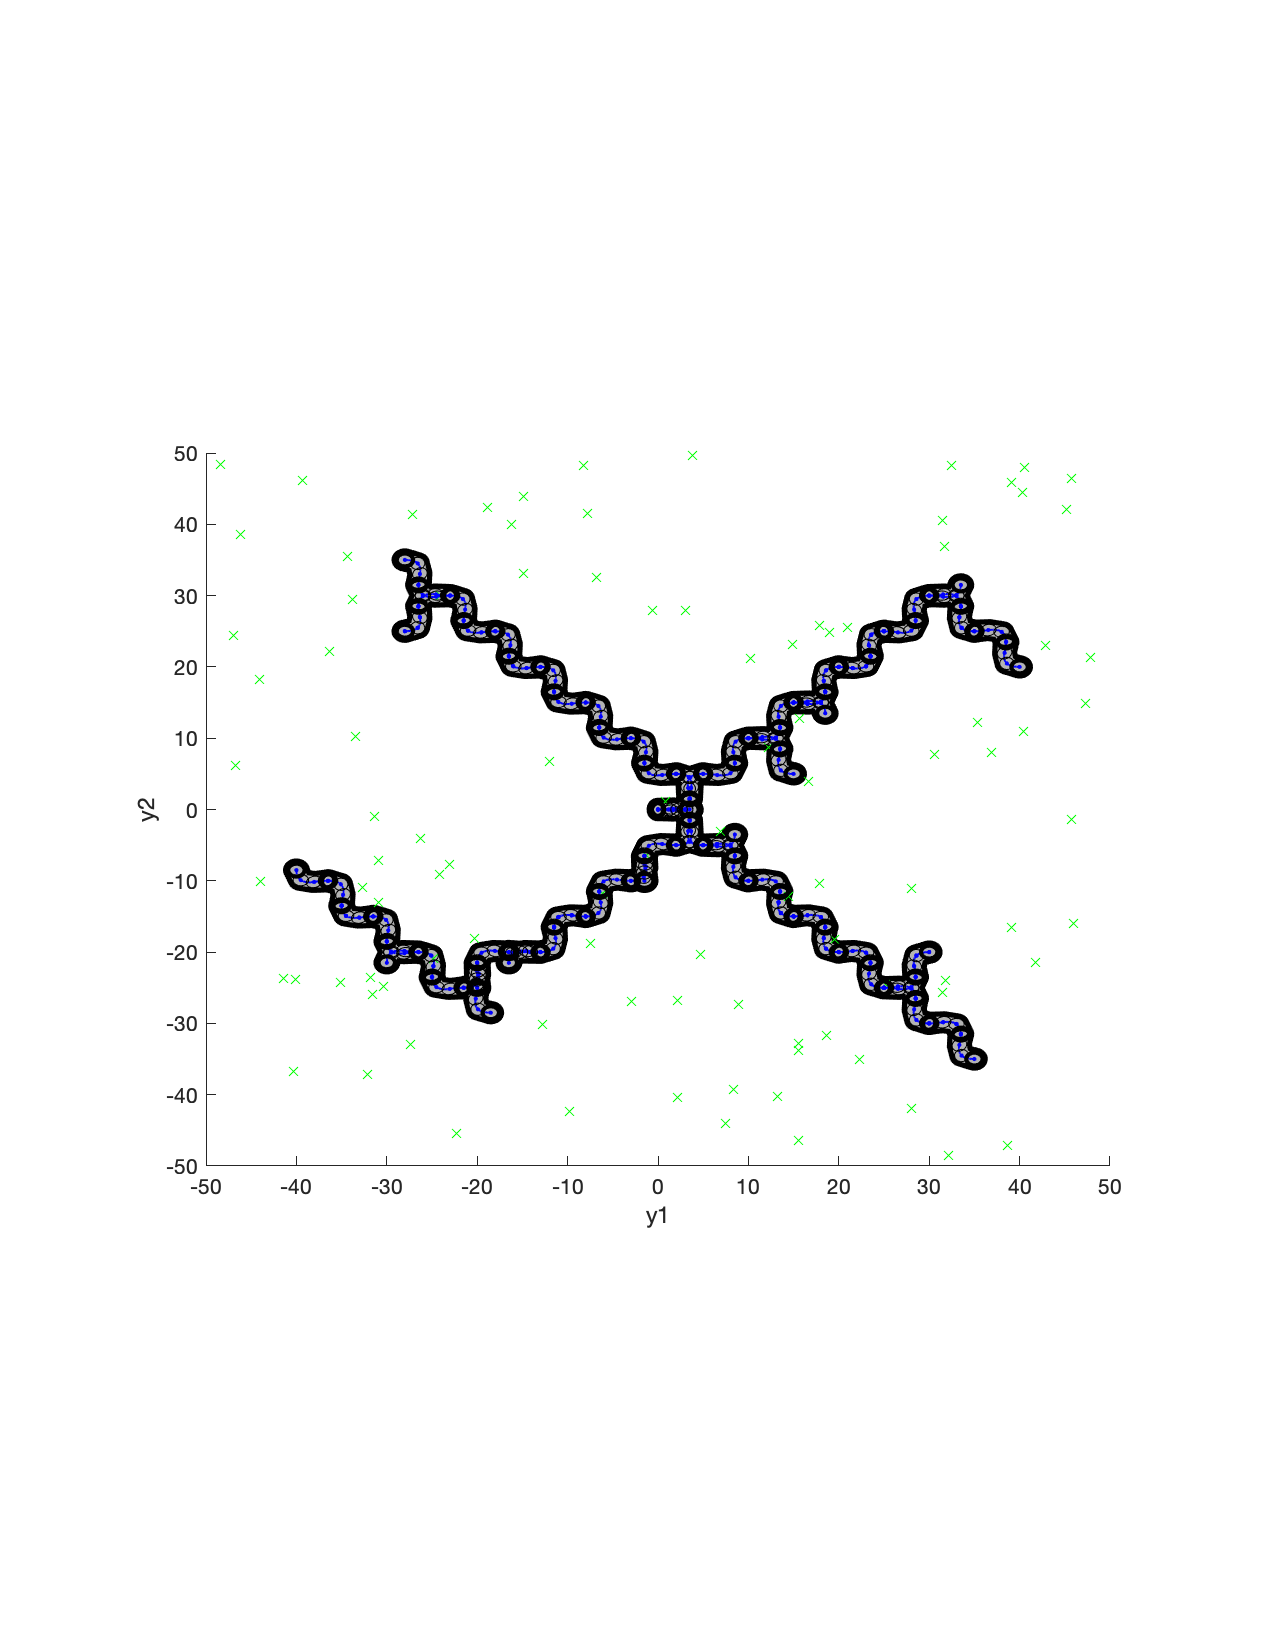
\includegraphics[scale=.5]{figures/rrtfunnel/rrtfunnel-modified-euclidean-100samples}
  \caption{The growth of the \textit{RRTFunnel} tree with three motion
    primitives, uniform sampling and the modified euclidean distance metric
    after 100 samples. The tree grows quickly into the open unexplored areas,
    like expected.}
\end{figure}

\begin{figure}
  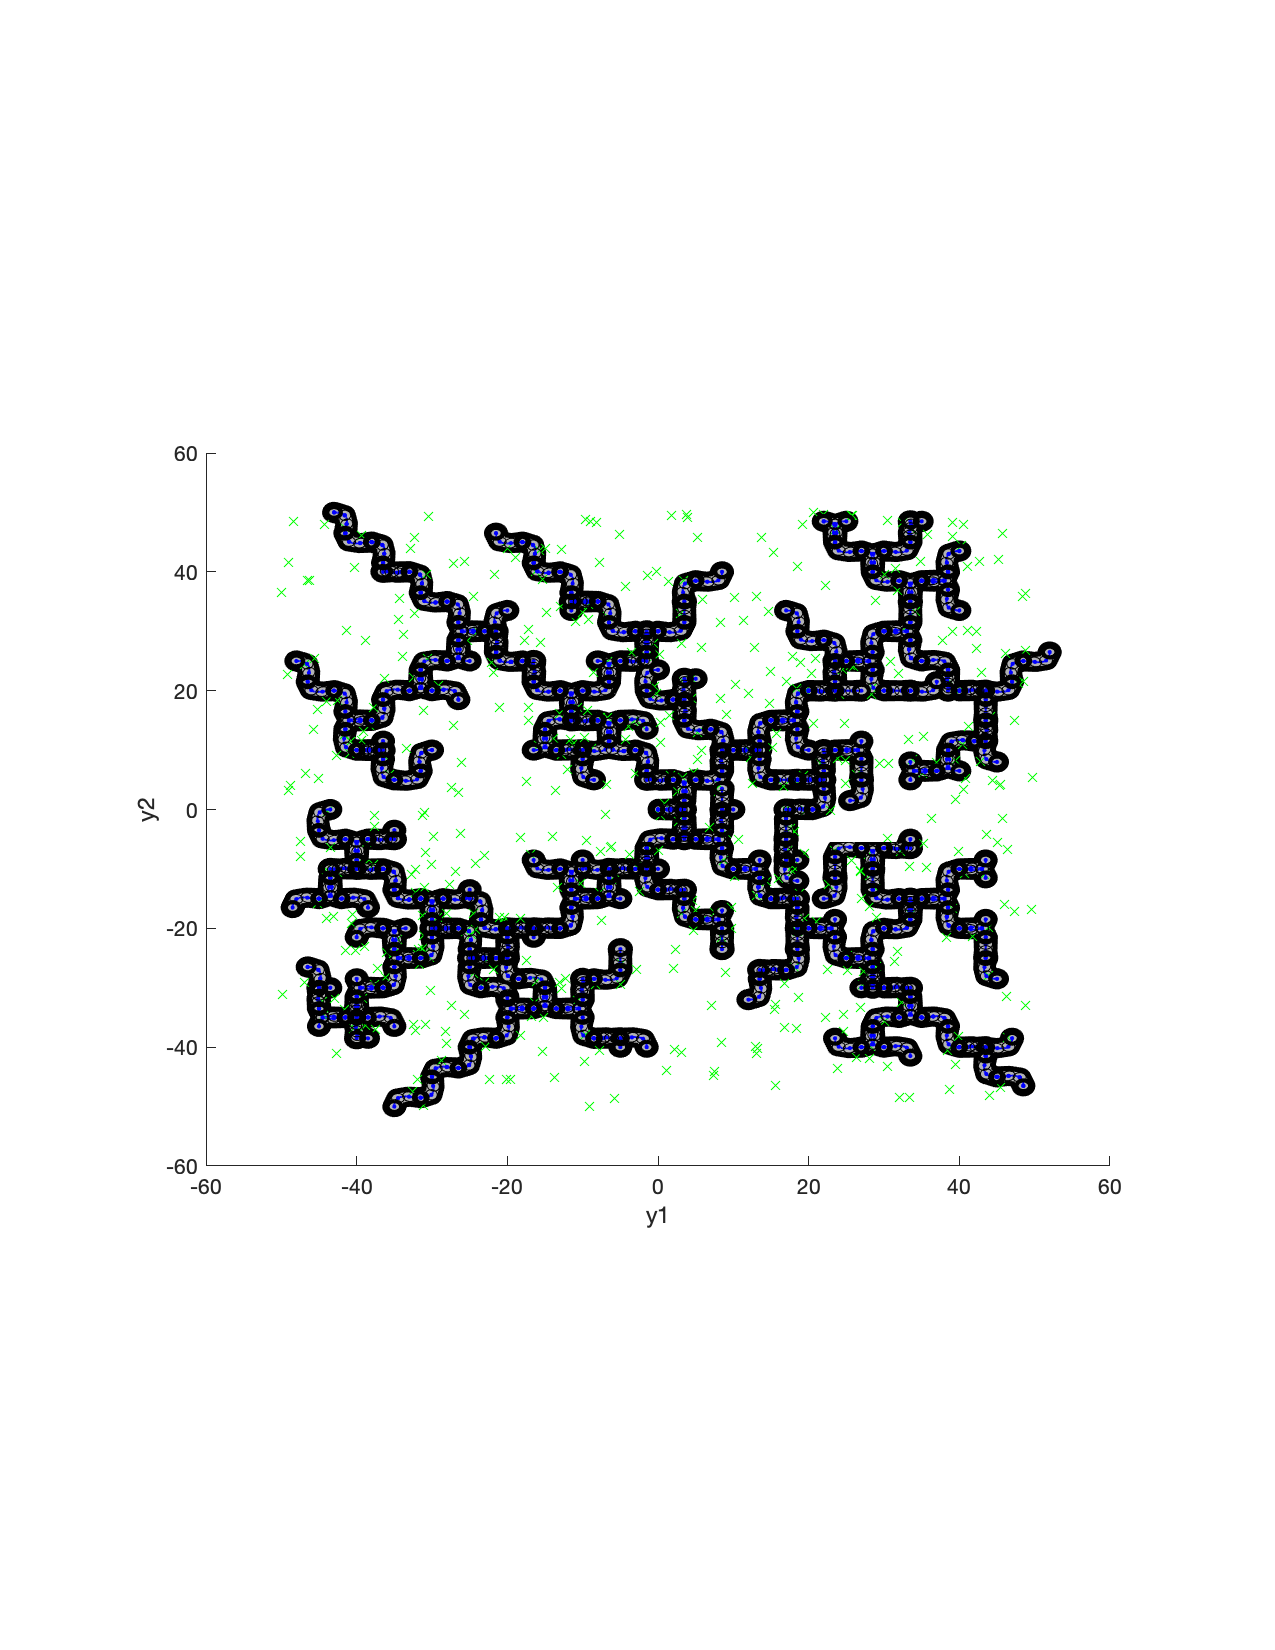
\includegraphics[scale=.5]{figures/rrtfunnel/rrtfunnel-modified-euclidean-500samples}
  \caption{The growth of the \textit{RRTFunnel} tree with three motion
    primitives, uniform sampling and the modified euclidean distance metric
    after 500 samples.}
\end{figure}

\begin{figure}
  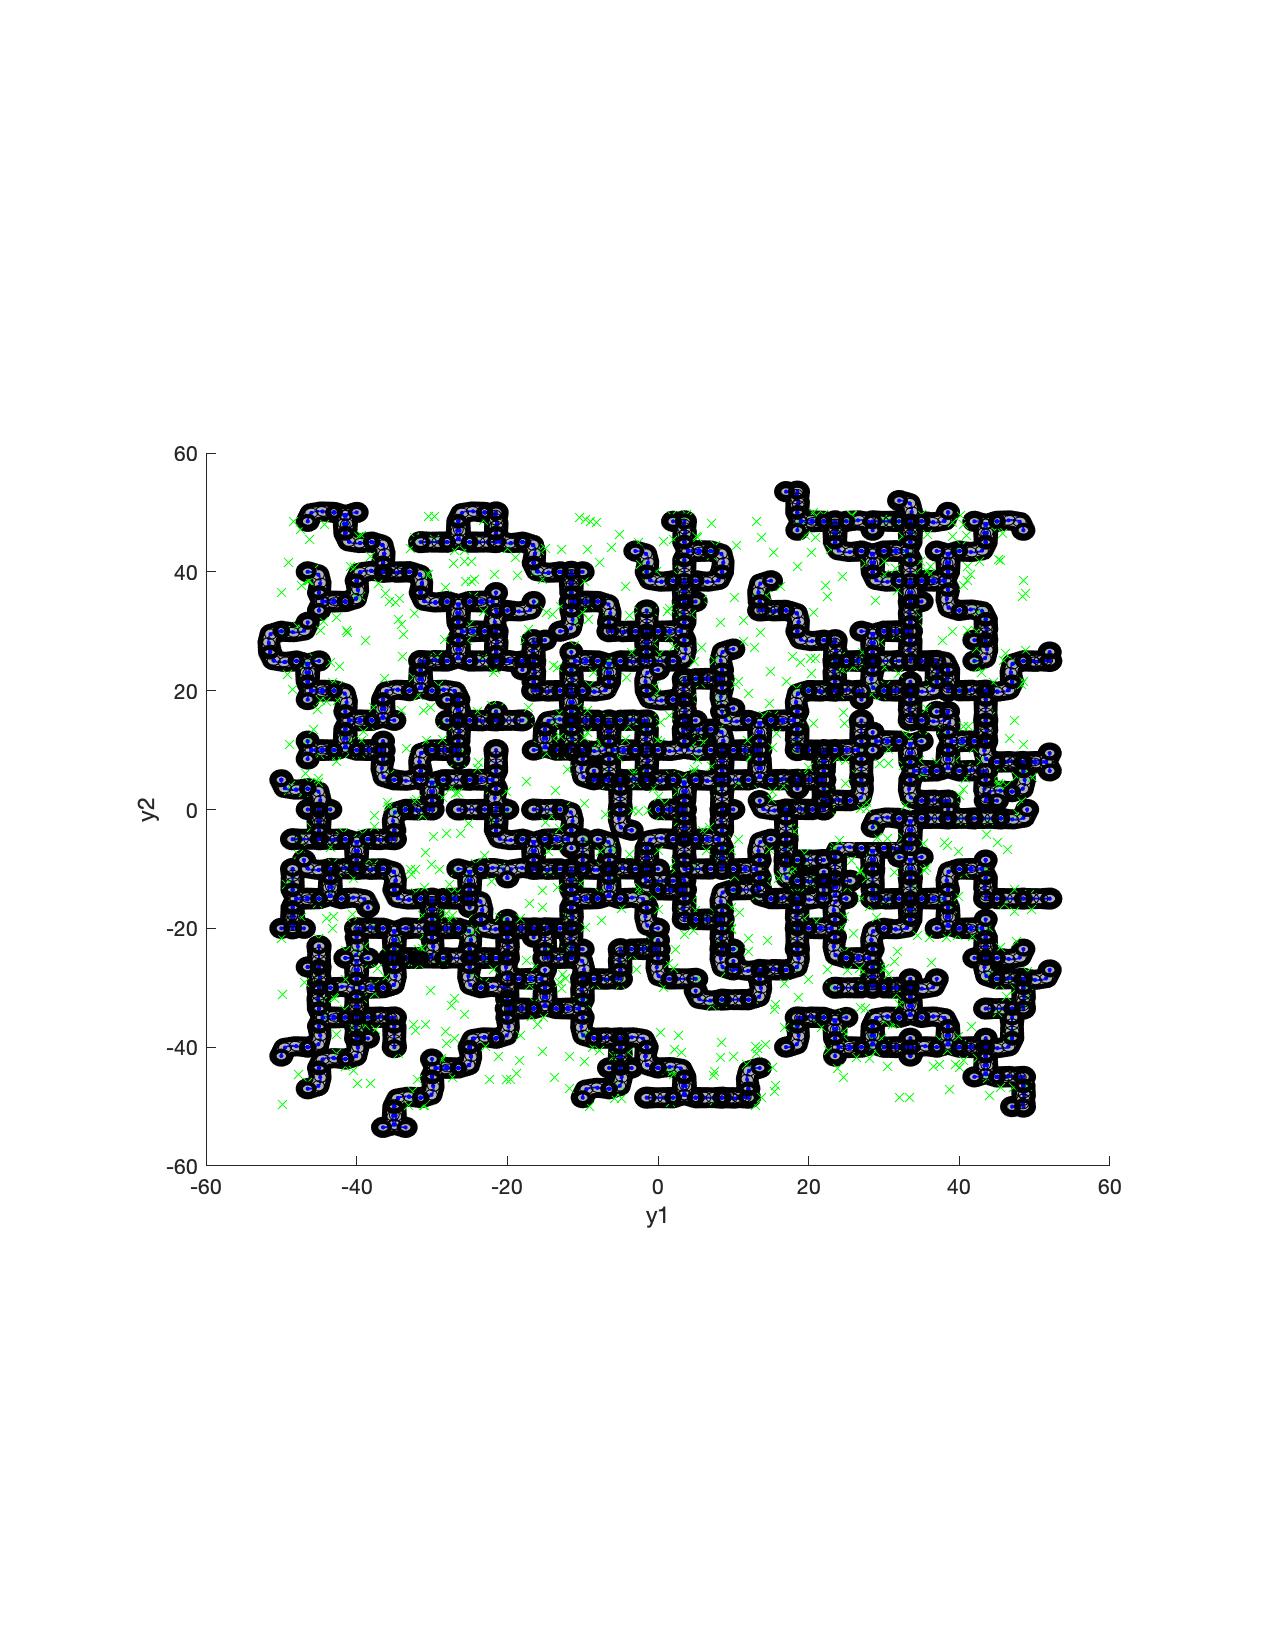
\includegraphics[scale=.5]{figures/rrtfunnel/rrtfunnel-modified-euclidean-1000samples}
  \caption{The growth of the \textit{RRTFunnel} tree with three motion
    primitives, uniform sampling and the modified euclidean distance metric
    after 1000 samples.}
\end{figure}


\subsection{Lyapunov function as a distance metric}
(TODO - is the lyapunov function a proper distance metric? It won't be symetric
will it?).

First test is with the lyapunov function used for validating the funnels in our
planner as a distance metric, however this was quickly abandoned after looking
at
\begin{figure}
  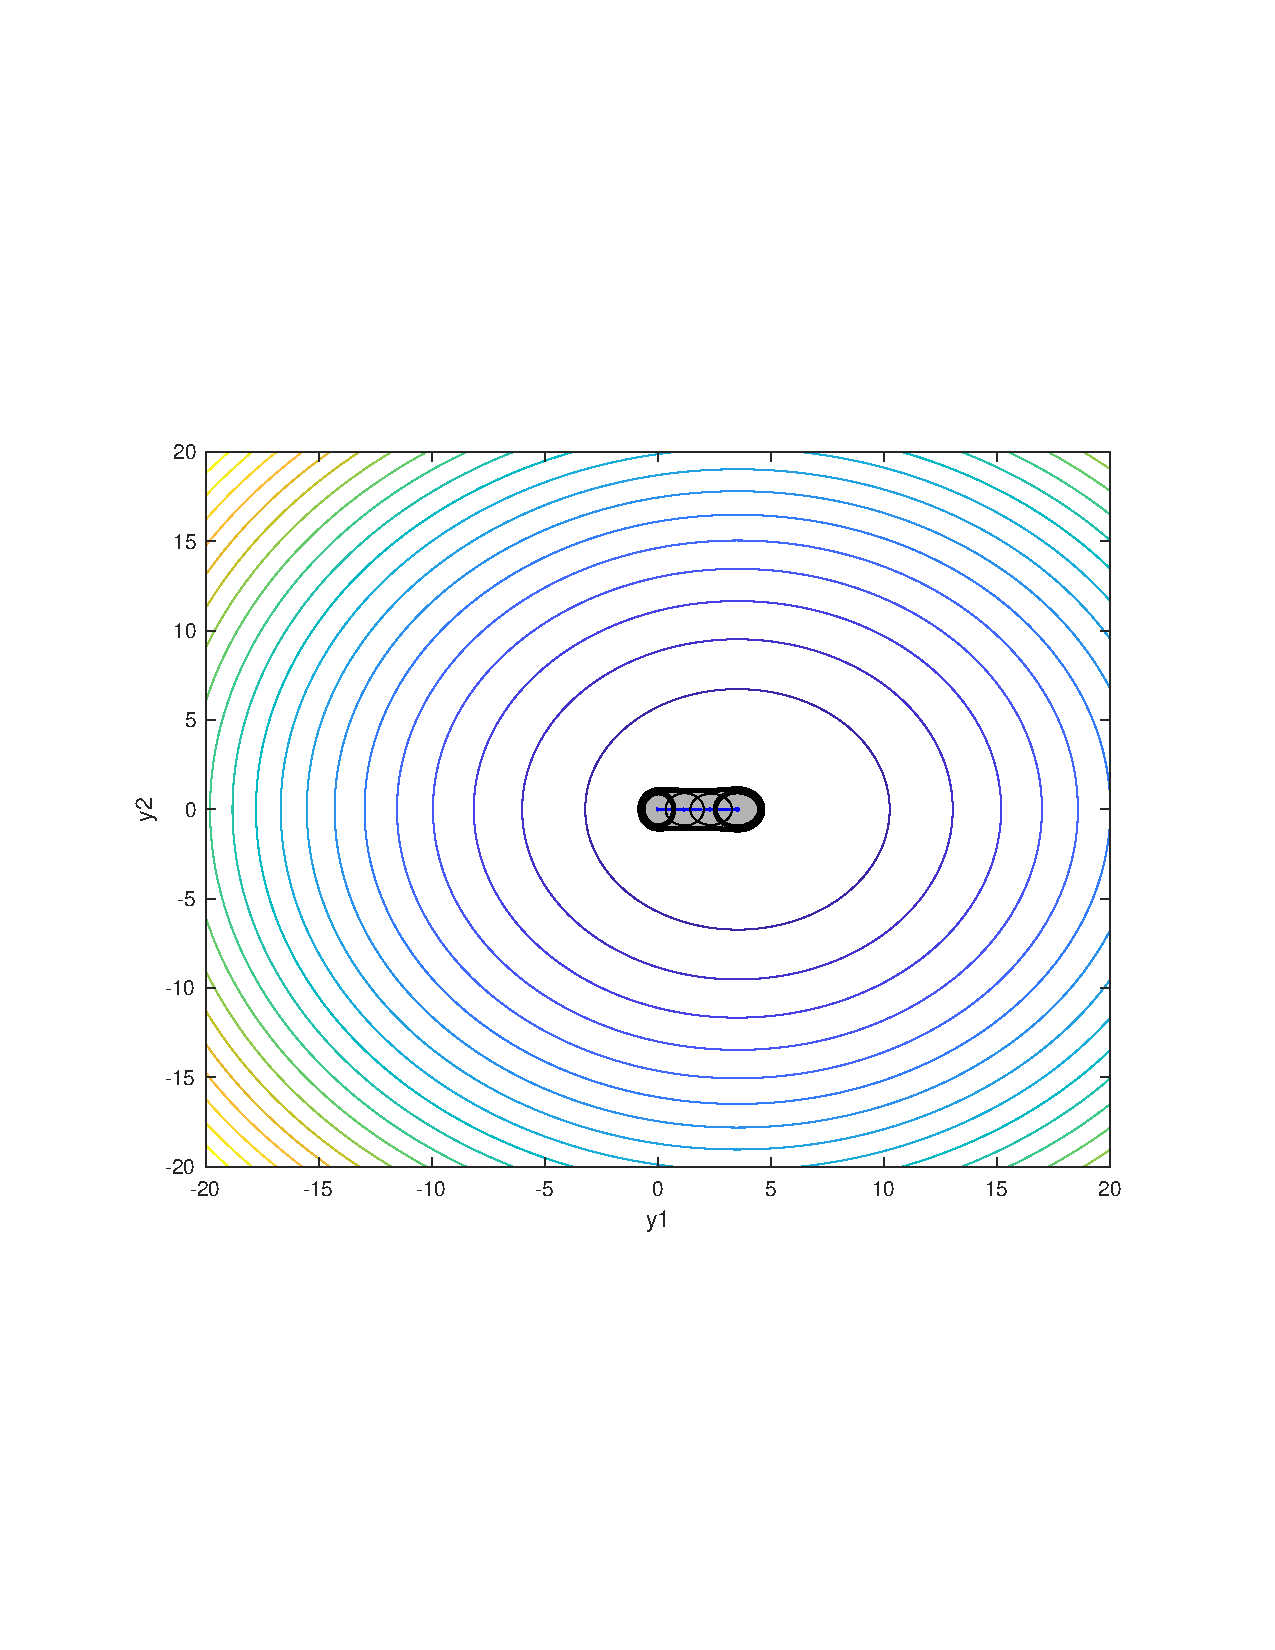
\includegraphics[scale=.5]{figures/rrtfunnel/straight-funnel-lyapunov-level-sets}
  \caption{The level sets of the quadratic Lyapunov function at the end of the
    straight funnel from the base set of the RRTFunnel algorithm.}
\end{figure}

\begin{figure}
  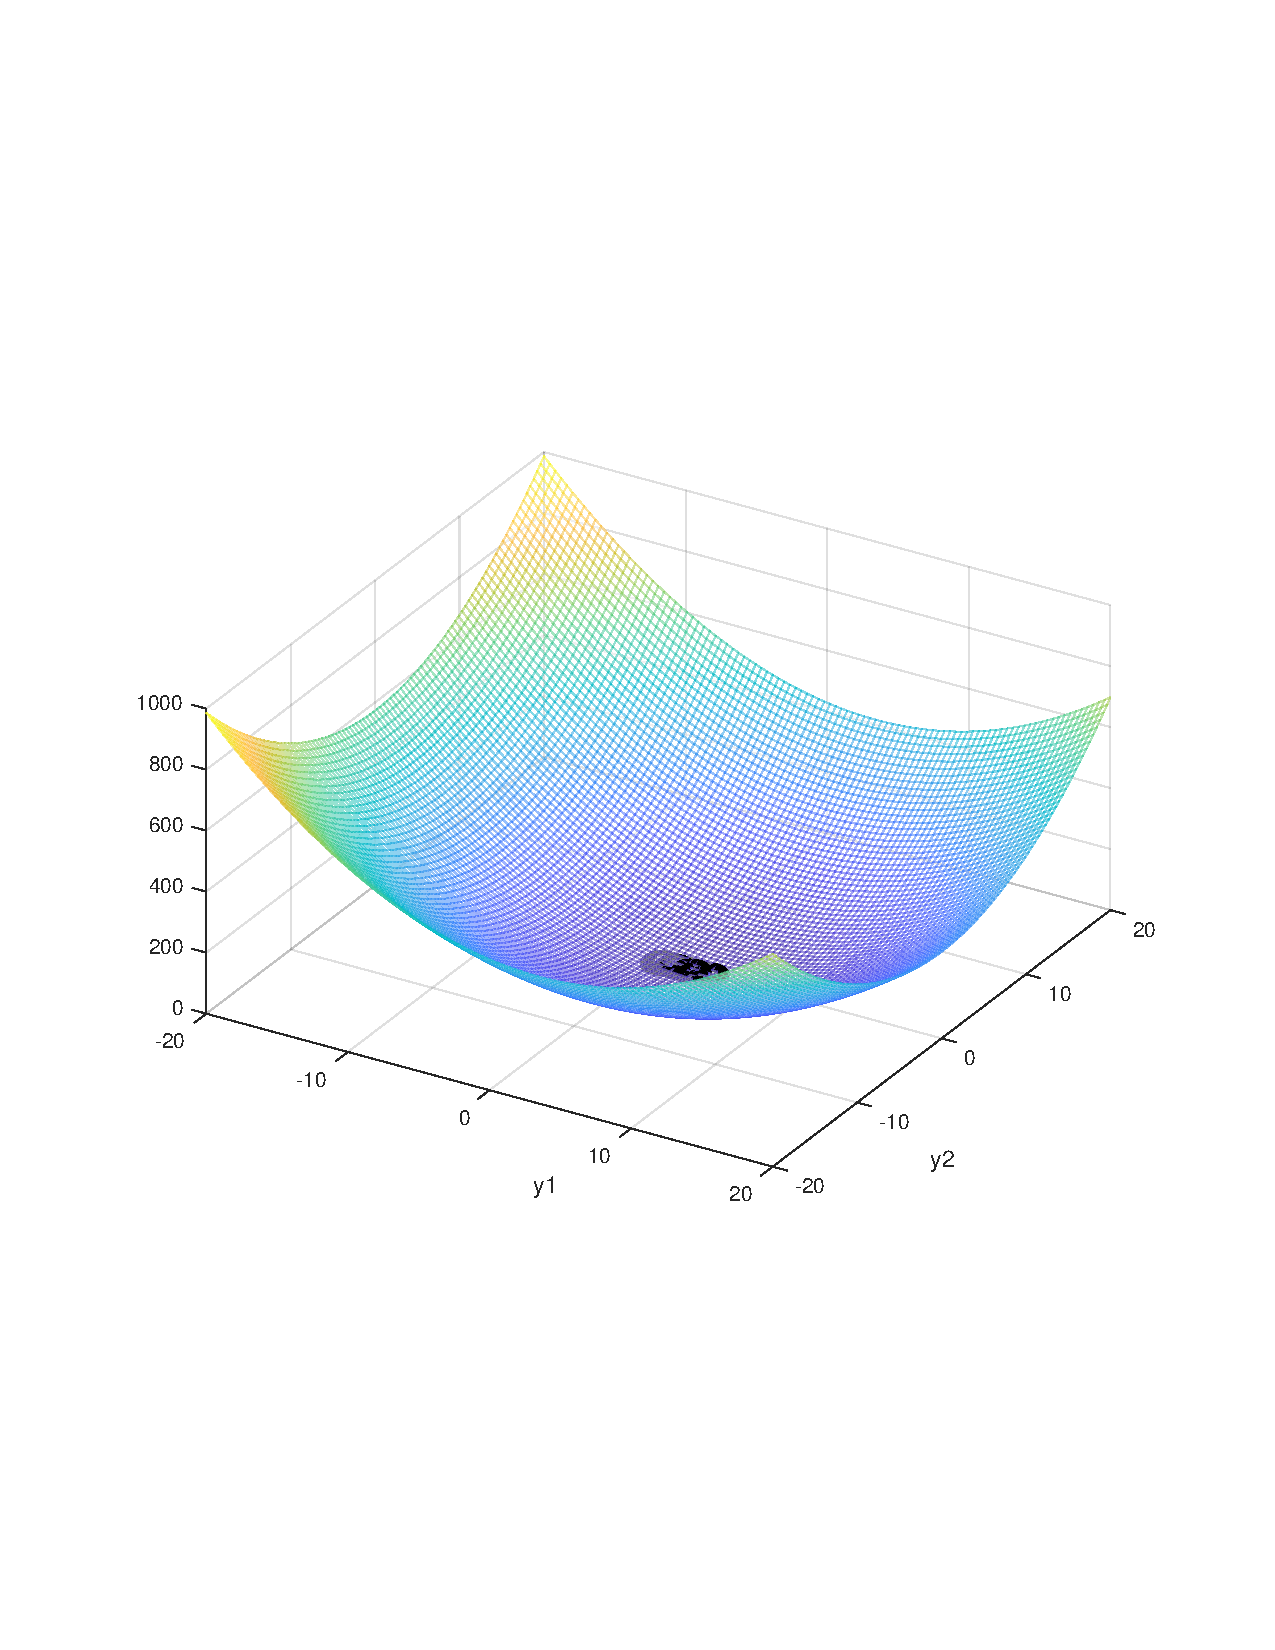
\includegraphics[scale=.5]{figures/rrtfunnel/straight-funnel-lyapunov-3d.pdf}
  \caption{The quadratic Lyapunov function visualized in 3D space for the
    straight funnel motion primitive.}
\end{figure}


The weaknesses of the Euclidean distance metric lead to the discovery of the
\cite{parkFeedbackMotionPlanning2015} paper, in which the authors use the
\textit{Lyapunov function} as a distance metric for the extension operator in an
optimal \textit{RRT*} algorithm.

In \cite{parkFeedbackMotionPlanning2015}, the lyapunov function is used as a
distance metric for the RRT algorithm. When this metric is applied to our
RRTFunnel algorithm, we get the following improvement upon the euclidean
distance metric. Using the same example as above:

% \begin{figure}
% \includegraphics{lyapunov-function-distance-closest-funnel}
% \end{figure}

% \begin{figure}
% \includegraphics{lyapunov-function-distance-extension-operator}
% \end{figure}

\section{Extending the motion primitive library}

Currently the motion primitive library has held only three motion primitives:
one straight forward motion, one left turn, and one right turn. Let's have a
look at how adding more motion primitives to our library will influence the
planner.

\subsection{Composing funnels}

Now that the library has more motion primitives, and not all of them end up with
the wheels straight ahead, and might even still have the wheels turning at the
end state, composing funnels requires a little more effort than just
translating one onto the end of the other. This can be done in two ways:
\begin{itemize}
  \item In real time as we are planning.
  \item Offline prior to planning, and then mark which funnels are compatible
    for extending eachother.
\end{itemize}